% This file was converted to LaTeX by Writer2LaTeX ver. 1.4
% see http://writer2latex.sourceforge.net for more info
\documentclass{report}

\usepackage[latin1]{inputenc}
\usepackage[T1]{fontenc}
\usepackage[english]{babel}
\usepackage{lmodern}
\usepackage{amsmath}
\usepackage{amssymb,amsfonts,textcomp}
\usepackage{array}
\usepackage{supertabular}
\usepackage{hhline}
\usepackage{graphicx}
\usepackage{listings}
\usepackage{geometry}

\geometry{
	a4paper,
	left=15mm,
	right=35mm,
	top=20mm,
	bottom=20mm,
}

\makeatletter
  \newcommand\arraybslash{\let\\\@arraycr}
\makeatother

\lstset{
	language=SQL,
	basicstyle=\ttfamily,
	xleftmargin=1cm
}

\setlength\tabcolsep{1mm}
\renewcommand\arraystretch{1.3}

\title{BSc2 - COMPUTING PROGRAMME}

\begin{document}
\begin{flushleft}
{\fontfamily{lmss}\selectfont

\clearpage

SQL WORKBOOK

\section[BSc Computing Programmes]{BSc Computing Programmes}
\section[5800 {}- DATABASE SYSTEMS]{5800 - DATABASE SYSTEMS}
\section[5440 {}- DATABASES FOR BUSINESS]{5440 - DATABASES FOR BUSINESS}

\section[2016 / 2017]{2016 / 2017}
This page is intentionally blank.

\clearpage
\section[BSc Computing Programme]{BSc Computing Programme}

\begin{center}

\begin{minipage}{13.25cm}
Contents by section

\begin{flushleft}
\tablefirsthead{}
\tablehead{}
\tabletail{}
\tablelasttail{}

\begin{supertabular}{m{2.1069999cm}m{1.433cm}m{21.439cm}}
Section & Page & Topics\\
\centering Intro & 3 & Oracle Application Express (APEX) system Sample tables\\
\centering A &
9

14 &
Using Oracle

About the exercises and SQL notation\\
\centering B &
15 &
SELECT {\dots} FROM {\dots} WHERE {\dots} ORDER BY

Simple arithmetic

Dates \& Time\\
\centering C &
27 &
Group functions:

\ \ sum, average, min and max

Using NULL, NVL

GROUP BY {\dots} HAVING\\
\centering D &
33 &
Simple Equi-joins

Non-equi joins\\
\centering E &
39 &
Data types, Naming rules 

CREATE tables

DROP table\\
 &
 &
INSERT data

Scripts\\
\centering F &
47 &
Table constraints

ALTERING tables

DELETE and UPDATE data\\
\centering G &
57 &
Table Alias names

Self joins

OUTER joins\\
\centering H &
63 &
Views and Sub-queries \\
\centering Appendix &
69 &
Oracle functions 

Indexes

Controlling access\\
 &
 &
\\
\end{supertabular}
\end{flushleft}
\end{minipage}
\end{center}

\begin{center}
\begin{minipage}{7.999cm}
Contents by topic

\begin{flushleft}
\tablefirsthead{}
\tablehead{}
\tabletail{}
\tablelasttail{}
\begin{supertabular}{m{5.051cm}m{2.299cm}}
\centering Topic &
\centering\arraybslash Section(s)\\
Accounting system

Alias\ \ (column)

\ \ (table)

ALTER 

CREATE

Data types

Dates

DELETE

DROP

Functions\ \ (simple)

\ \ \ \ (group)

\ \ \ \ (reference)

GROUP BY{\dots}.HAVING

INSERT &
Introduction

B

G

F

E

E

B

E

E

B

C

Appendix

C

E\\
JOIN\ \ (simple)

\ \ (equi-)

\ \ (self-)

\ \ (outer-)

NULL\ \ (and functions)

\ \ (in joins)

ORDER BY

Personnel System

SELECT &
D

D

G

G

C

F

C

Introduction

B\\
Subqueries

UPDATE

VIEW

WHERE &
H

E

H

B\\
\end{supertabular}
\end{flushleft}
\end{minipage}
\end{center}
\begin{center}
\begin{minipage}{6.525cm}
Find key material in video: youtube.com/user/cboisvert2


\includegraphics[width=4.911cm,height=4.77cm]{images/img (1).png}
 
\end{minipage}
\end{center}
\clearpage
References:

Ben Forta - SAMS Teach Yourself SQL in 10 minutes -- 4th Edition

Colin Ritchie - Database Principles and Design - 3rd Edition

Connolly, Begg \& Strachan - Database Systems  {}-  5th Edition

ORACLE OCP Introduction to Oracle9i:SQL Exam Guide (Exam 1Z0-007) 

The Page Header references throughout the workbook provide a broad pointer to the pages relating to the workbook material.

Note: Topics must be completed in order, each may use material/skills developed in a previous section.  Topics must be completed before the scheduled session of the next topic.

\clearpage
\chapter{INTRODUCTION}
Relational Database Systems should be easy to understand and to use.

But it is not always convenient, or possible, to control them visually through a graphical interface.

Instead most relational database systems use a standard, written language to control the database and to access the data: SQL (the {\textquotedbl}Structured Query Language{\textquotedbl}).

Commands are typed a line at a time (at a {\textquotedbl}command line interface{\textquotedbl}) or saved in files to be executed in succession (in {\textquotedbl}batch{\textquotedbl}). It may surprise you if you are accustomed to graphical interfaces, rather than typed commands, but SQL is designed to be easy to learn and use.

The commands are interpreted by a Database Management System (DBMS), usually running remotely on a server, to carry out the necessary functions. Here are some main functionalities and words used:

\ \ {}- Create and modify a database structure: CREATE, DROP, ALTER

\ \ {}- Operate on the data: SELECT, INSERT, UPDATE, DELETE 

\ \ {}- Control who can access a database: GRANT, REVOKE

One of the features that make SQL easy to use is that the language is declarative. This means that SQL contains the necessary commands to describe what you want to be done, but not how it should be done.

For example this SQL command:

\ \ SELECT * FROM EMPLOYEE;

Means {\textquotedbl}find every row and every column from the employee table{\textquotedbl}. As you can see, the command focuses on the essentials (what you want) and ignores all the detail of procedure (what the system will do to get it).

The details -{}-{}-exactly which files should be opened to find the data, how to look into them-{}-{}- are left entirely to the Database Management System, which executes the commands accurately and efficiently so we can focus on the data, rather than the technology. Most of the time, we will be able to work on the data and its structure while keeping the details of how a DBMS manages it all for another day.

There are many database systems available. This booklet will teach you SQL by practicing on one of the best known DBMSs: Oracle. Being a relational database system, it holds data in tables.

Before the work begins, the next two pages describe the data that the booklet uses for example queries.

\clearpage
\section{SAMPLE TABLES}
Oracle creates and populates a set of default tables (EMP, DEPT and SALGRADE) for all new users. These are the Personnel System. All of the Exercises throughout this workbook are based on the Personnel System tables.

Should data in the personnel tables become corrupt, they may be restored to their original status by issuing each of the following statements for the appropriate table:

\ \ DROP TABLE EMP ;

\ \ CREATE TABLE EMP AS SELECT * FROM EXAMPLE.EMP ;

\subsection{The Personnel System}
\subsubsection[Table: \ EMP]{Table:  EMP}
\begin{flushleft}
\tablefirsthead{}
\tablehead{}
\tabletail{}
\tablelasttail{}
\begin{supertabular}{|m{1.8cm}|m{2.0509999cm}|m{2.55cm}|m{1.301cm}|m{2.3009999cm}|m{1.798cm}|m{1.74cm}|m{1.858cm}|}
\hline
\centering EMPNO &
\centering ENAME &
\centering JOB &
\centering MGR &
\centering HIREDATE &
\centering SAL &
\centering COMM &
\centering\arraybslash DEPTNO\\\hline
 &
 &
 &
 &
 &
 &
 &
\\
\centering 7369 &
SMITH &
CLERK &
\centering 7902 &
17-DEC-80 &
\raggedleft 800.00 &
 &
\centering\arraybslash 20\\
\centering 7499 &
ALLEN &
SALESMAN &
\centering 7698 &
20-FEB-81 &
\raggedleft 1600.00 &
\raggedleft 300.00 &
\centering\arraybslash 30\\
\centering 7521 &
WARD &
SALESMAN &
\centering 7698 &
22-FEB-81 &
\raggedleft 1250.00 &
\raggedleft 500.00 &
\centering\arraybslash 30\\
\centering 7566 &
JONES &
MANAGER &
\centering 7839 &
02-APR-81 &
\raggedleft 2975.00 &
 &
\centering\arraybslash 20\\
\centering 7654 &
MARTIN &
SALESMAN &
\centering 7698 &
28-SEP-81 &
\raggedleft 1200.00 &
\raggedleft 1250.00 &
\centering\arraybslash 30\\
\centering 7698 &
BLAKE &
MANAGER &
\centering 7839 &
01-MAY-81 &
\raggedleft 2850.00 &
 &
\centering\arraybslash 30\\
\centering 7782 &
CLARK &
MANAGER &
\centering 7839 &
09-JUN-81 &
\raggedleft 2450.00 &
 &
\centering\arraybslash 10\\
\centering 7788 &
SCOTT &
ANALYST &
\centering 7566 &
09-DEC-82 &
\raggedleft 3000.00 &
 &
\centering\arraybslash 20\\
\centering 7839 &
KING &
PRESIDENT &
 &
17-NOV-81 &
\raggedleft 5000.00 &
 &
\\
\centering 7844 &
TURNER &
SALESMAN &
\centering 7698 &
08-SEP-81 &
\raggedleft 1500.00 &
\raggedleft 0.00 &
\centering\arraybslash 30\\
\centering 7876 &
ADAMS &
CLERK &
\centering 7788 &
12-JAN-83 &
\raggedleft 1100.00 &
 &
\centering\arraybslash 20\\
\centering 7900 &
JAMES &
CLERK &
\centering 7698 &
03-DEC-81 &
\raggedleft 950.00 &
 &
\centering\arraybslash 30\\
\centering 7902 &
FORD &
ANALYST &
\centering 7566 &
03-DEC-81 &
\raggedleft 3000.00 &
 &
\centering\arraybslash 20\\
\centering 7934 &
MILLER &
CLERK &
\centering 7782 &
23-JAN-82 &
\raggedleft 1300.00 &
 &
\centering\arraybslash 10\\\hline
\end{supertabular}
\end{flushleft}
\subsubsection[Table: \ DEPT]{Table:  DEPT}
\begin{flushleft}
\tablefirsthead{}
\tablehead{}
\tabletail{}
\tablelasttail{}
\begin{supertabular}{|m{2.047cm}|m{3.3009999cm}|m{2.802cm}|}
\hline
\centering DEPTNO &
\centering DNAME &
\centering\arraybslash LOC\\\hline
 &
 &
\\
\centering 10 &
ACCOUNTING &
NEW YORK\\
\centering 20 &
RESEARCH &
DALLAS\\
\centering 30 &
SALES &
CHICAGO\\
\centering 40 &
OPERATIONS &
BOSTON\\\hline
\end{supertabular}
\end{flushleft}
\subsubsection[Table: \ SALGRADE]{Table:  SALGRADE}
\begin{flushleft}
\tablefirsthead{}
\tablehead{}
\tabletail{}
\tablelasttail{}
\begin{supertabular}{|m{2.049cm}|m{2.552cm}|m{2.299cm}|}
\hline
\centering GRADE &
\centering LOSAL &
\centering\arraybslash HISAL\\\hline
 &
 &
\\
\centering 1 &
\raggedleft 700.00 &
\raggedleft\arraybslash 1200.00\\
\centering 2 &
\raggedleft 1201.00 &
\raggedleft\arraybslash 1400.00\\
\centering 3 &
\raggedleft 1401.00 &
\raggedleft\arraybslash 2000.00\\
\centering 4 &
\raggedleft 2001.00 &
\raggedleft\arraybslash 3000.00\\
\centering 5 &
\raggedleft 3001.00 &
\raggedleft\arraybslash 9999.00\\\hline
\end{supertabular}
\end{flushleft}
Several worked examples in this book are based on part of an Accounting System. They use three tables, CUST, CUSTACC and ACC. These tables represent the fact that a customer may have many accounts, and that an account may be held jointly by more than one customer. Details of these tables follow. 

The accounting system is not installed in your account; you will create it later in the book, but until you do, you can't test queries that use it, only work out what they would do.

\begin{center}

\includegraphics[width=1.06cm,height=0.903cm]{images/img (2).png}

\end{center}
\subsection{The Accounting System}

\begin{center}
\begin{minipage}{3.694cm}
CUST
\end{minipage}
\end{center}
\begin{center}
\begin{minipage}{3.694cm}
ACC
\end{minipage}
\end{center}
\begin{center}
\begin{minipage}{3.81cm}
CUSTACC
\end{minipage}
\end{center}
\begin{minipage}{2.515cm}
Allocated
\end{minipage}
\begin{center}
\begin{minipage}{1.997cm}
Owns
\end{minipage}
\end{center}

Table:  CUST

\begin{flushleft}
\tablefirsthead{}
\tablehead{}
\tabletail{}
\tablelasttail{}
\begin{supertabular}{|m{2.2389998cm}|m{2.55cm}|m{4.053cm}|m{2.799cm}|}
\hline
REFNO &
NAME &
ADDRESS &
AREA\\\hline
A123 &
J Doe &
1 High Street &
Sheffield\\
A124 &
J Smith &
2 West Street &
Sheffield\\
B127 &
R Best &
4 East Row &
Rotherham\\
B128 &
J Best &
4 East Row &
Rotherham\\
C371 &
R Done &
23 Middle Avenue &
Barnsley\\\hline
\end{supertabular}
\end{flushleft}
Table:  CUSTACC

\begin{flushleft}
\tablefirsthead{}
\tablehead{}
\tabletail{}
\tablelasttail{}
\begin{supertabular}{|m{2.3009999cm}|m{2.299cm}|}
\hline
REFNO &
ACCNO\\\hline
A123 &
1245890\\
A123 &
1494315\\
B127 &
5418490\\
B128 &
5418490\\\hline
\end{supertabular}
\end{flushleft}
Table:  ACC

\begin{flushleft}
\tablefirsthead{}
\tablehead{}
\tabletail{}
\tablelasttail{}
\begin{supertabular}{|m{2.3009999cm}|m{2.486cm}|m{2.8cm}|m{2.799cm}|m{2.802cm}|}
\hline
ACCNO &
BALANCE &
BRANCH &
OPENED &
BONUS\\\hline
1245890 &
\raggedleft 234.50 &
Broomhill &
12 Nov 2003 &
\raggedleft\arraybslash 100.00\\
1494315 &
\raggedleft 0.50 &
Tinsley &
15 Dec 1999 &
\raggedleft\arraybslash 0.00\\
5418490 &
\raggedleft 1789.40 &
Broomhill &
6 May 1988 &
\\\hline
\end{supertabular}
\end{flushleft}
This page is intentionally blank.

\clearpage



\chapter{SQL Lab Week 1}
\section{Objectives}
\begin{itemize}
\item Create an Oracle User for yourself.
\item Gain access to the Oracle system.
\item Meet the APEX Oracle environment 
\item Practice entering and running simple statements (without understanding them in detail)
\item Gain an exposure to error messages.
\end{itemize}
\section{Creating your User in ORACLE }
All students must register as an Oracle User.  For this you will need:

\begin{itemize}
\item your Student Number
\item your personal details
\end{itemize}
Start https://dbutils.shu.ac.uk/oracleutility  or from the Start menu



\begin{center}
  
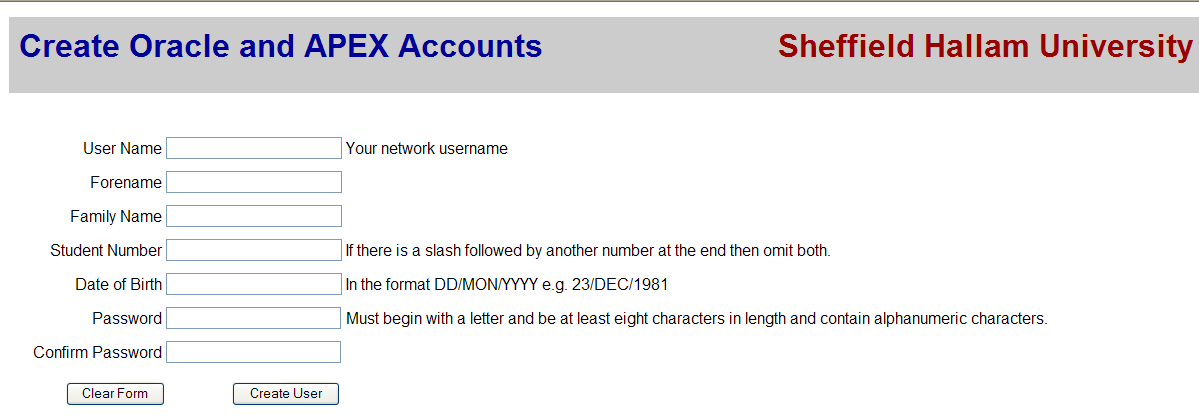
\includegraphics[width=13.201cm,height=4.574cm]{images/img (3).png}

\end{center}
\begin{center}
\begin{minipage}{4.177cm}
Enter your Log-in Id, Name and Student Number
\end{minipage}
\end{center}


\begin{center}
\begin{minipage}{4.177cm}
The format for Date of Birth is

dd/mmm/yyyy, e.g. 01/JAN/1990
\end{minipage}
\end{center}


\begin{center}
\begin{minipage}{14.441cm}
Choose a password (that you will remember!). The password rules:

\begin{itemize}
\item eight characters in length
\item start with a letter
\item the remainder may be letters or numbers
\item Oracle passwords are NOT case sensitive
\end{itemize}
\end{minipage}
\end{center}
Click the 'Create User' button, and wait. Interrupting the process can corrupt your Oracle details and you may not be able to re-run the process. If successful you now have a personal and private Oracle environment and two accounts: for Oracle, the DBMS, and for APEX, the Web front-end. Both use the same username and password. The database has been populated with the three Personnel Systems tables that we will use throughout the semester.

If you did not get an account, check that the format of your entries is correct. Does the University know you by different personal details? If your name, or your date of birth, is recorded by the University with a typo, enter it here with

\begin{center}
  

\includegraphics[width=1.06cm,height=0.903cm]{images/img (2).png}

\end{center}
the same typo. If you still don't seem to get an account, ask for help -- we'll ensure you do.

\clearpage 
\section{Starting Oracle}
Once you have your account, access the APEX facility via  one of the following paths:

Start Menu/Programs/Specialist Applications/Oracle/Application Express Login/

or:

http://homepages.shu.ac.uk:7777/pls/apex

You will be prompted for your Oracle User Code and Workspace (use your username for both) and your Oracle Password.



\begin{center}
  
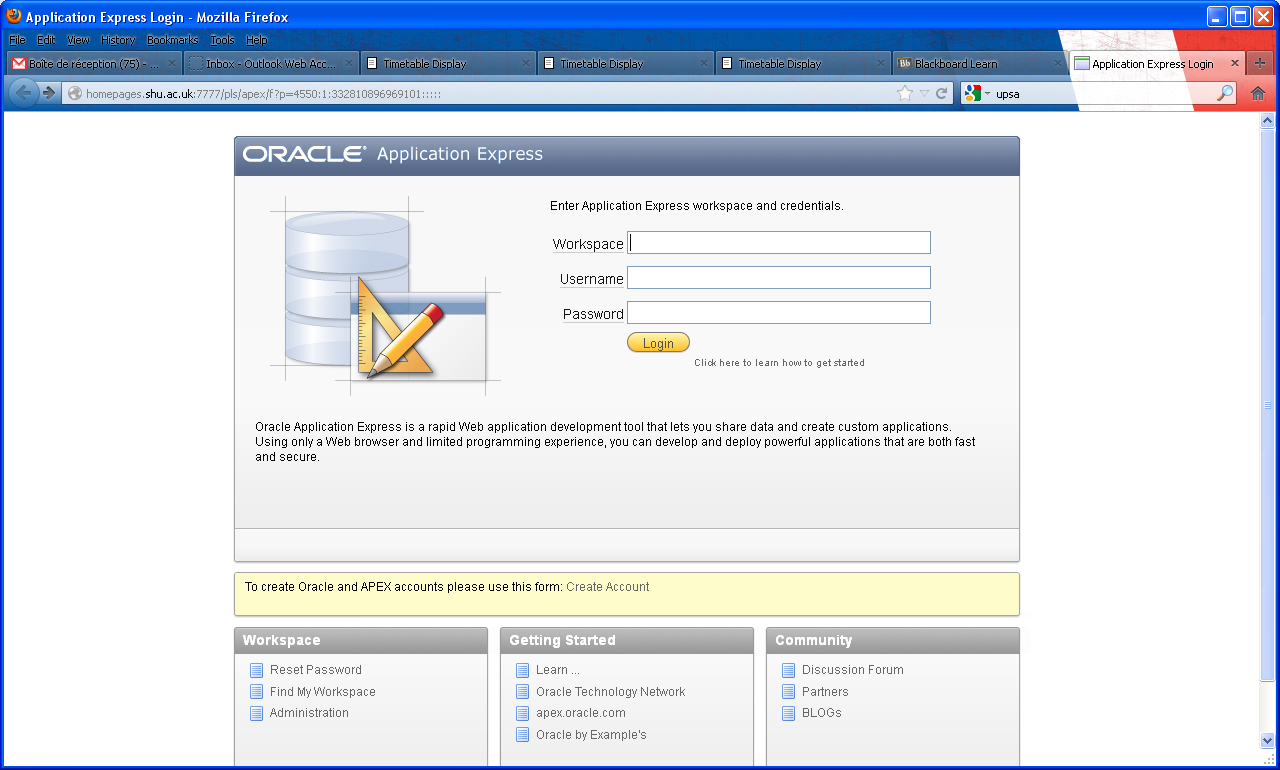
\includegraphics[width=9.479cm,height=3.41cm]{images/img (4).png}

\end{center}
\begin{center}
\begin{minipage}{4.092cm}
Workspace and Username are the same, enter it twice
\end{minipage}
\end{center}
Oracle will present you with APEX web interface.

\begin{center}
\begin{minipage}{3.958cm}
Select 

SQL Workshop
\end{minipage}
\end{center}


\begin{center}
  
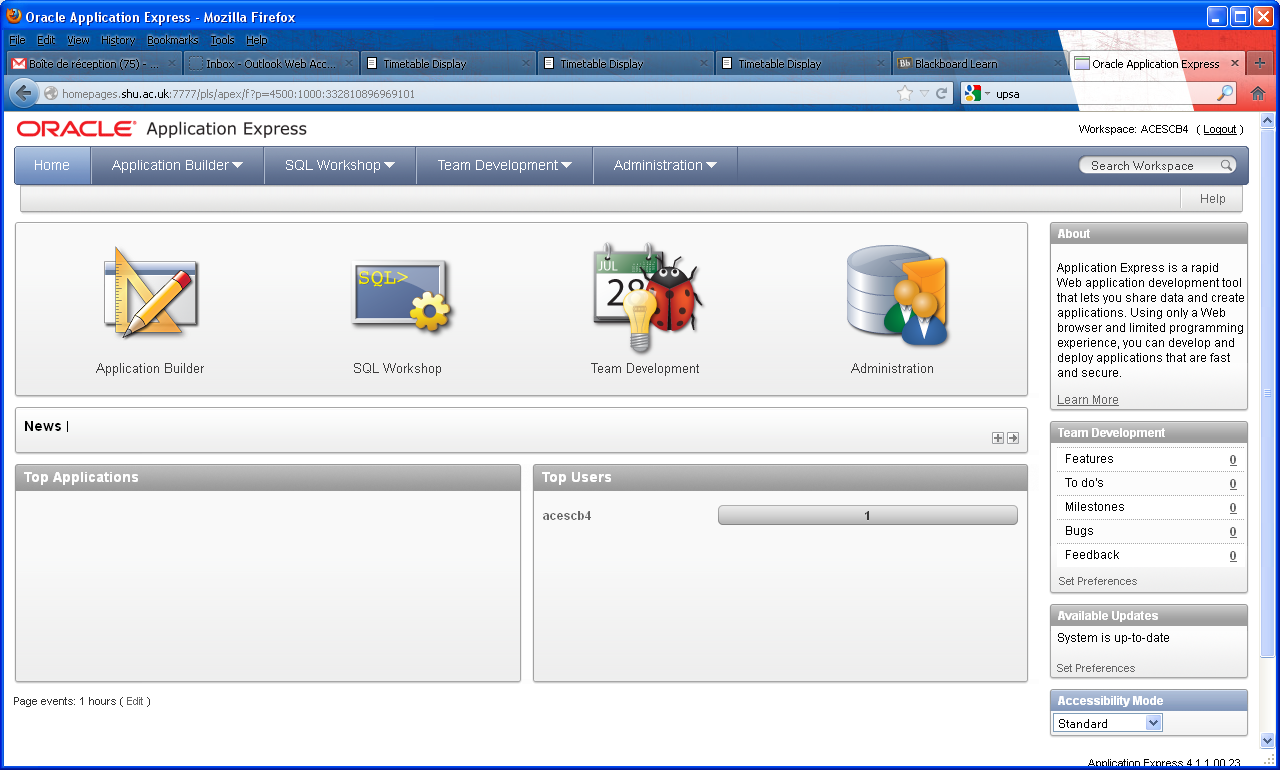
\includegraphics[width=13.028cm,height=3.478cm]{images/img (5).png}

\end{center}
The screen now shows four features. During this module you will use the first three:



\begin{center}
  
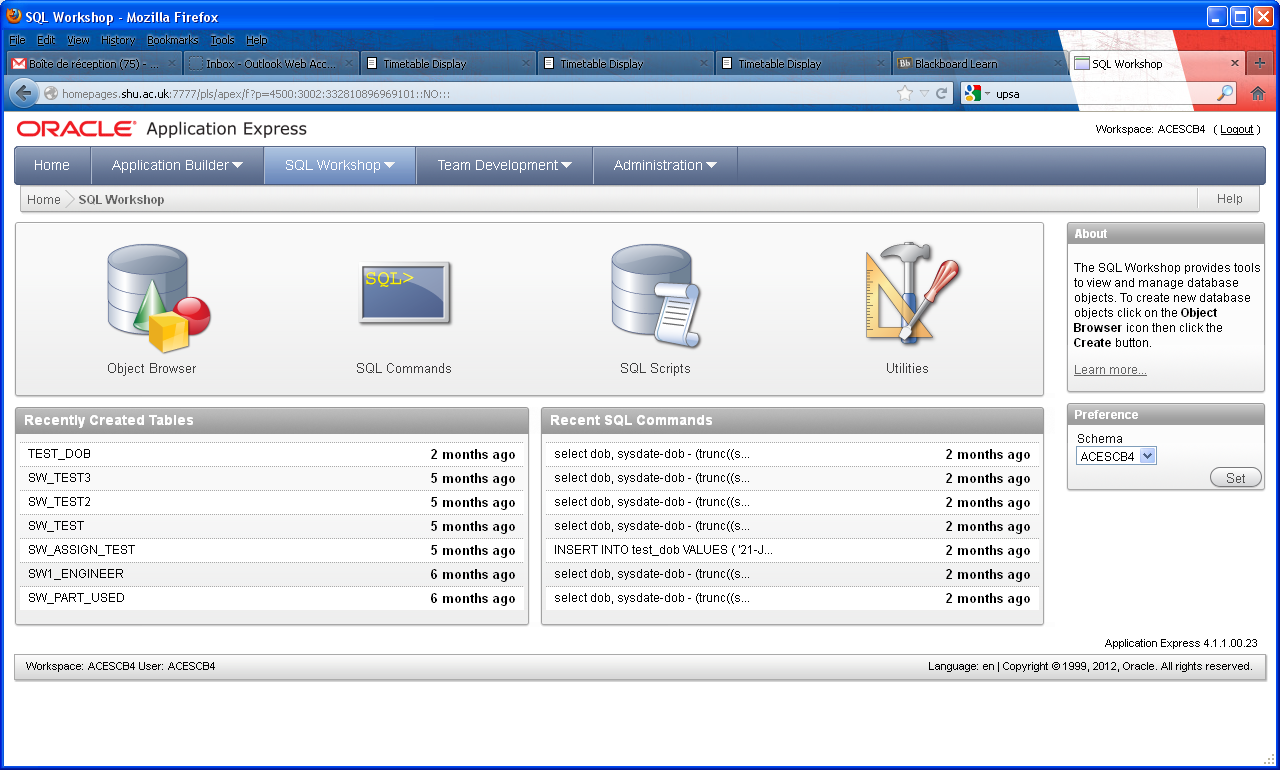
\includegraphics[width=13.162cm,height=2.436cm]{images/img (6).png}

\end{center}


\begin{center}
\begin{minipage}{6.368cm}
SQL Scripts:

save commands to execute (or re-execute) later, or save multiple commands to execute in batch.
\end{minipage}
\end{center}
\begin{center}
\begin{minipage}{4.189cm}
SQL Commands: 

type SQL that is immediately executed;
\end{minipage}
\end{center}
\begin{center}
\begin{minipage}{3.981cm}
Object Browser:

explore the tables and other objects forming your database
\end{minipage}
\end{center}
By the end of this Lab session you will have tried all three of them.

Select the SQL Commands feature. A two part screen will be displayed.

\begin{center}
  
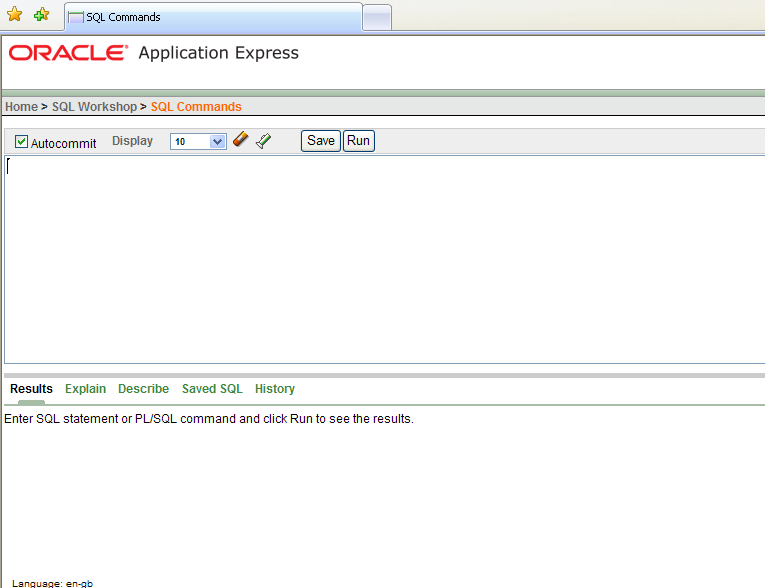
\includegraphics[width=13.728cm,height=10.4cm]{images/img (7).png}

\end{center}


\begin{center}
\begin{minipage}{4.584cm}
Save statements to check or re-run later
\end{minipage}
\end{center}
\begin{center}
\begin{minipage}{4.246cm}
Display option:  controls how many results are displayed (check it: are some rows not displayed?)
\end{minipage}
\end{center}


\begin{center}
\begin{minipage}{2.789cm}
Clear Command (eraser); remove the current statement

\end{minipage}
\end{center}
\begin{center}
\begin{minipage}{4.706cm}
Top section: enter your statements here.
\end{minipage}
\end{center}


\begin{center}
\begin{minipage}{4.944cm}
Lower section: the results of running that statement.
\end{minipage}
\end{center}
You are now ready to issue SQL statements.

\section{First steps}
\begin{itemize}
\item 
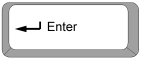
\includegraphics[width=1.63cm,height=0.683cm]{images/img (8).png}
  is the Enter key on the keyboard 
\end{itemize}
\begin{itemize}
\item After entering each statement click the 
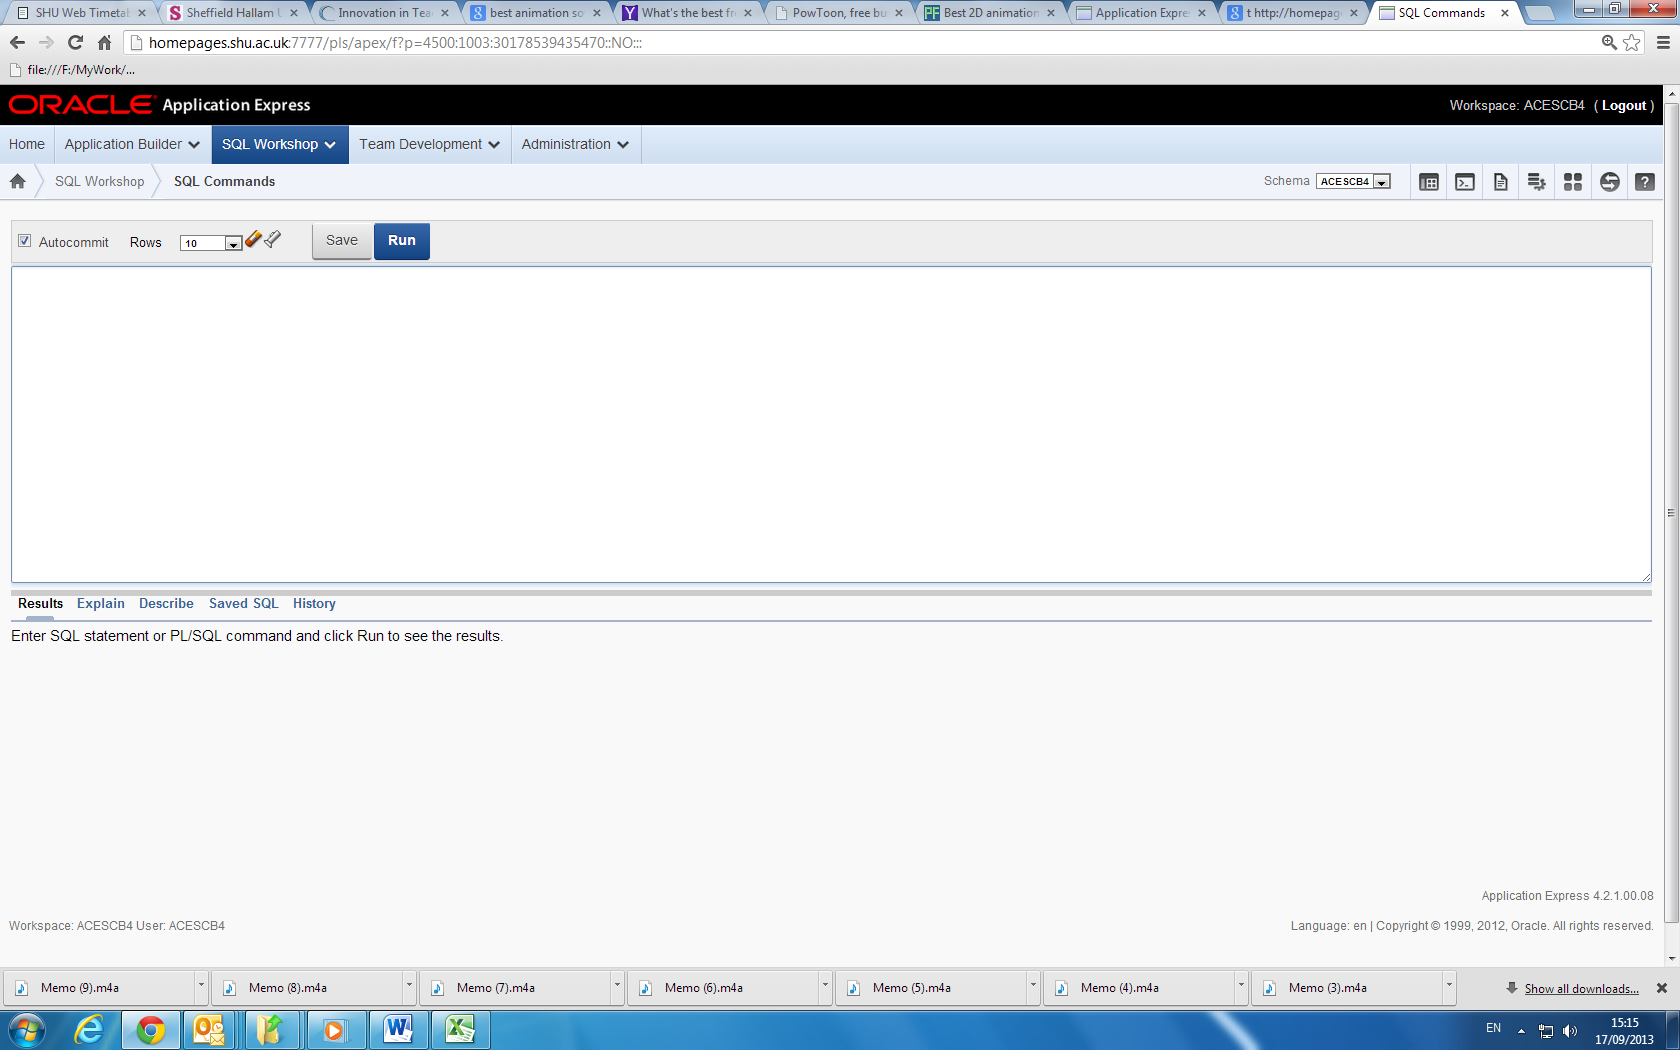
\includegraphics[width=0.947cm,height=0.607cm]{images/img (9).png}
  button. 
\end{itemize}
\begin{itemize}
\item Study the results and, for each group of statements, write down your conclusions.
\end{itemize}
\begin{itemize}
\item Now type in the following commands or statements exactly as presented
\end{itemize}
Try this:

SELECT  *  from EMP; 
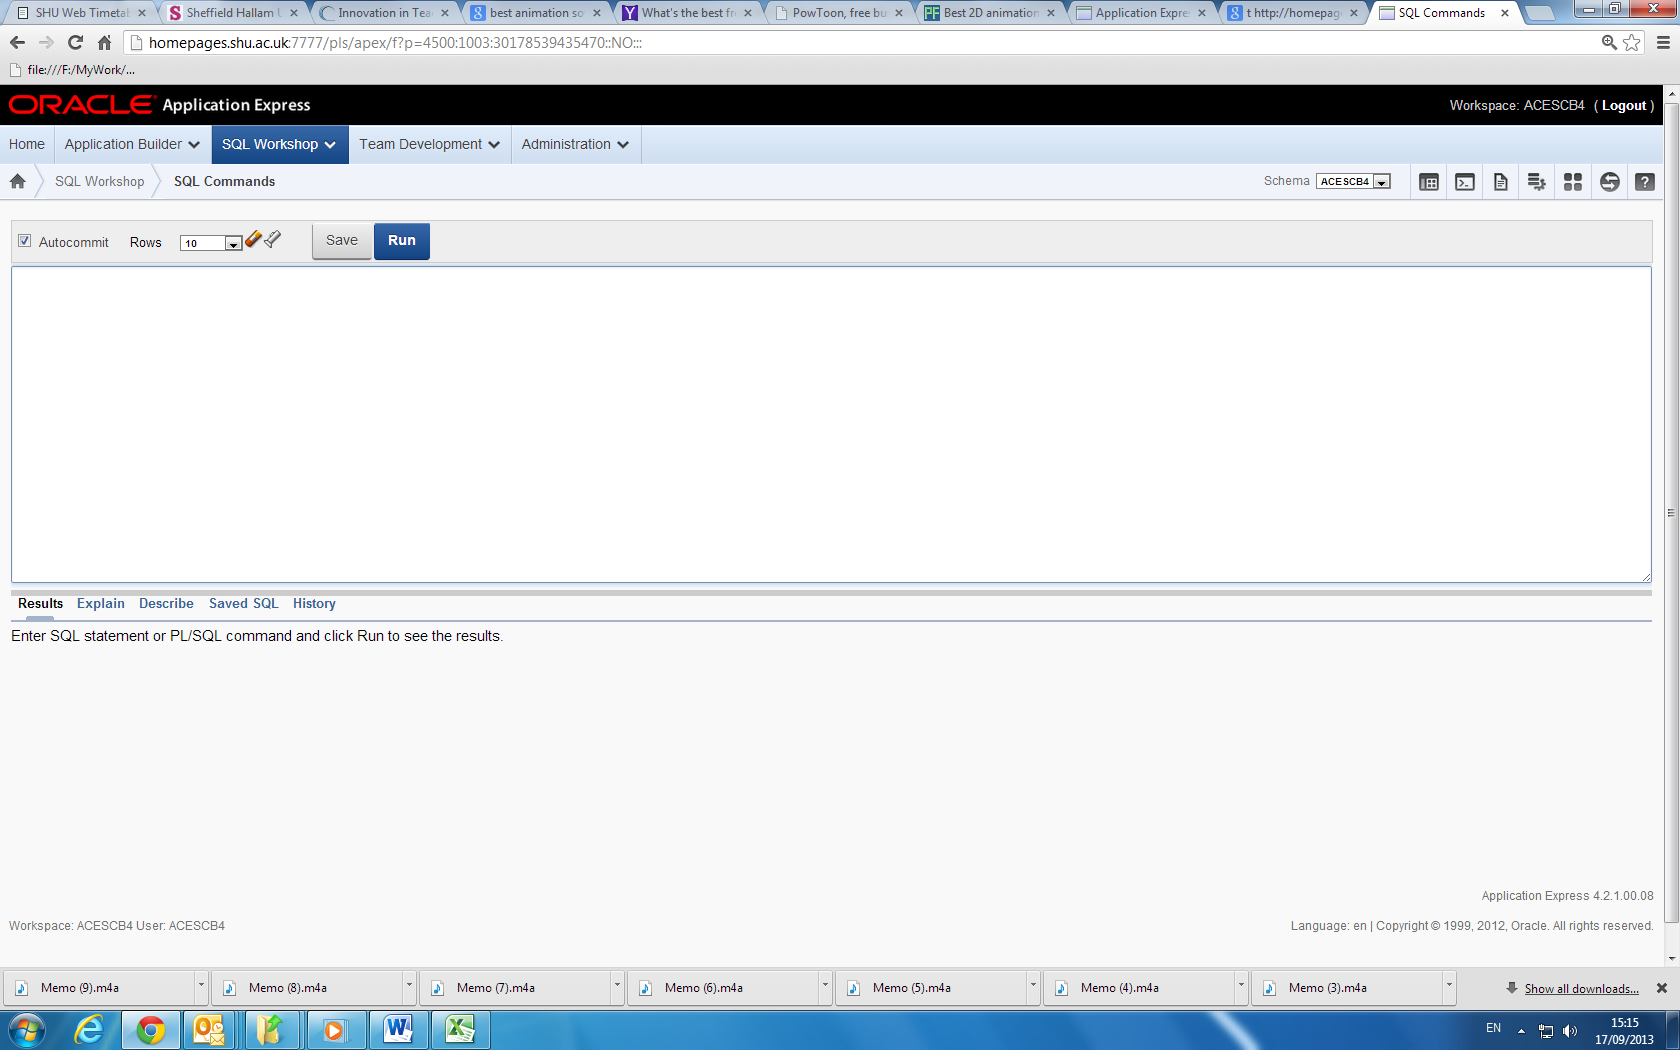
\includegraphics[width=0.947cm,height=0.607cm]{images/img (9).png}
 

The command should return the contents of the EMP table (example result over the page).

Oracle (helpfully?) makes the semi-colon optional for single statements, though it is the standard. These rules vary between database vendors: the {\textquotedbl}safe{\textquotedbl} approach is to follow the standard, and always use a semi-colon.

\begin{center}
  

\includegraphics[width=1.058cm,height=0.903cm]{images/img (2).png}

\end{center}
   
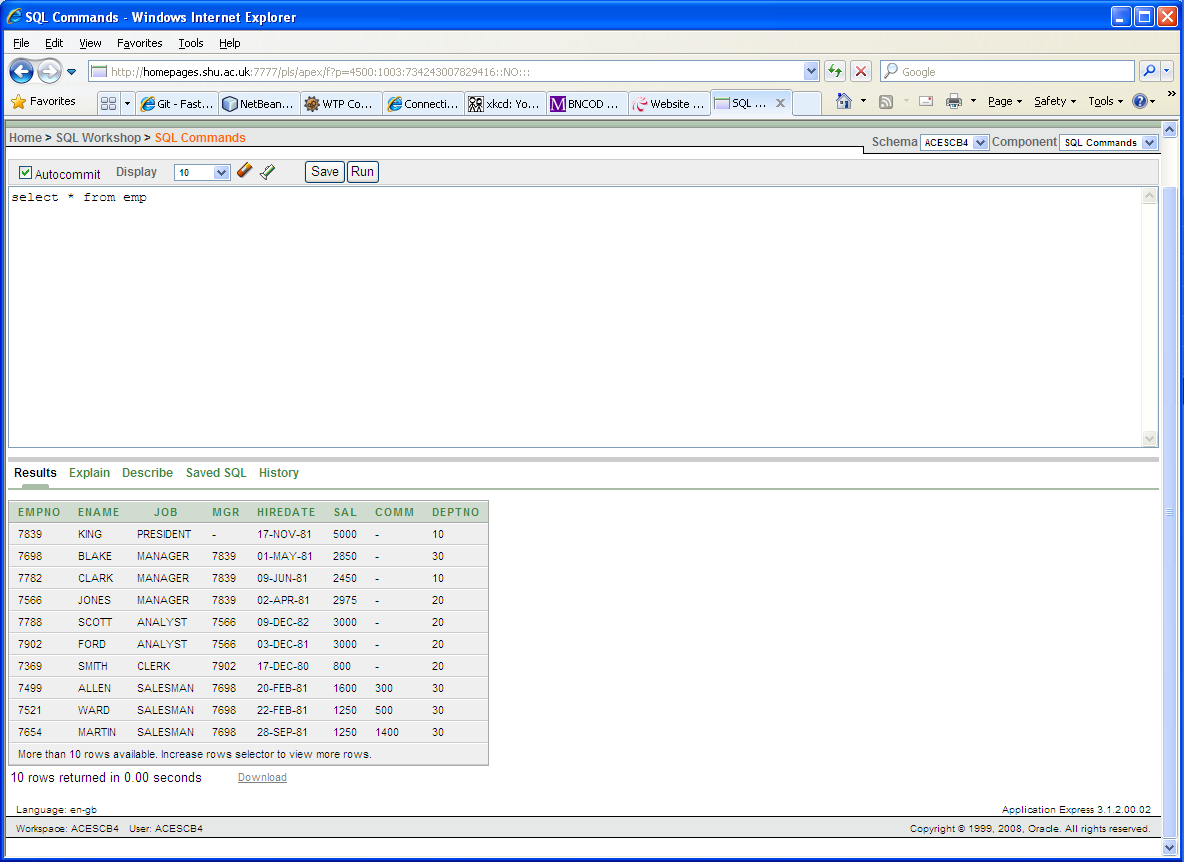
\includegraphics[width=14.785cm,height=8.871cm]{images/img (10).png}
 

Now try these alternatives, one at a time. Clear the upper part of the screen before entering each one:

Do lower case commands work? Clear the last command and type

select  *  from emp; 
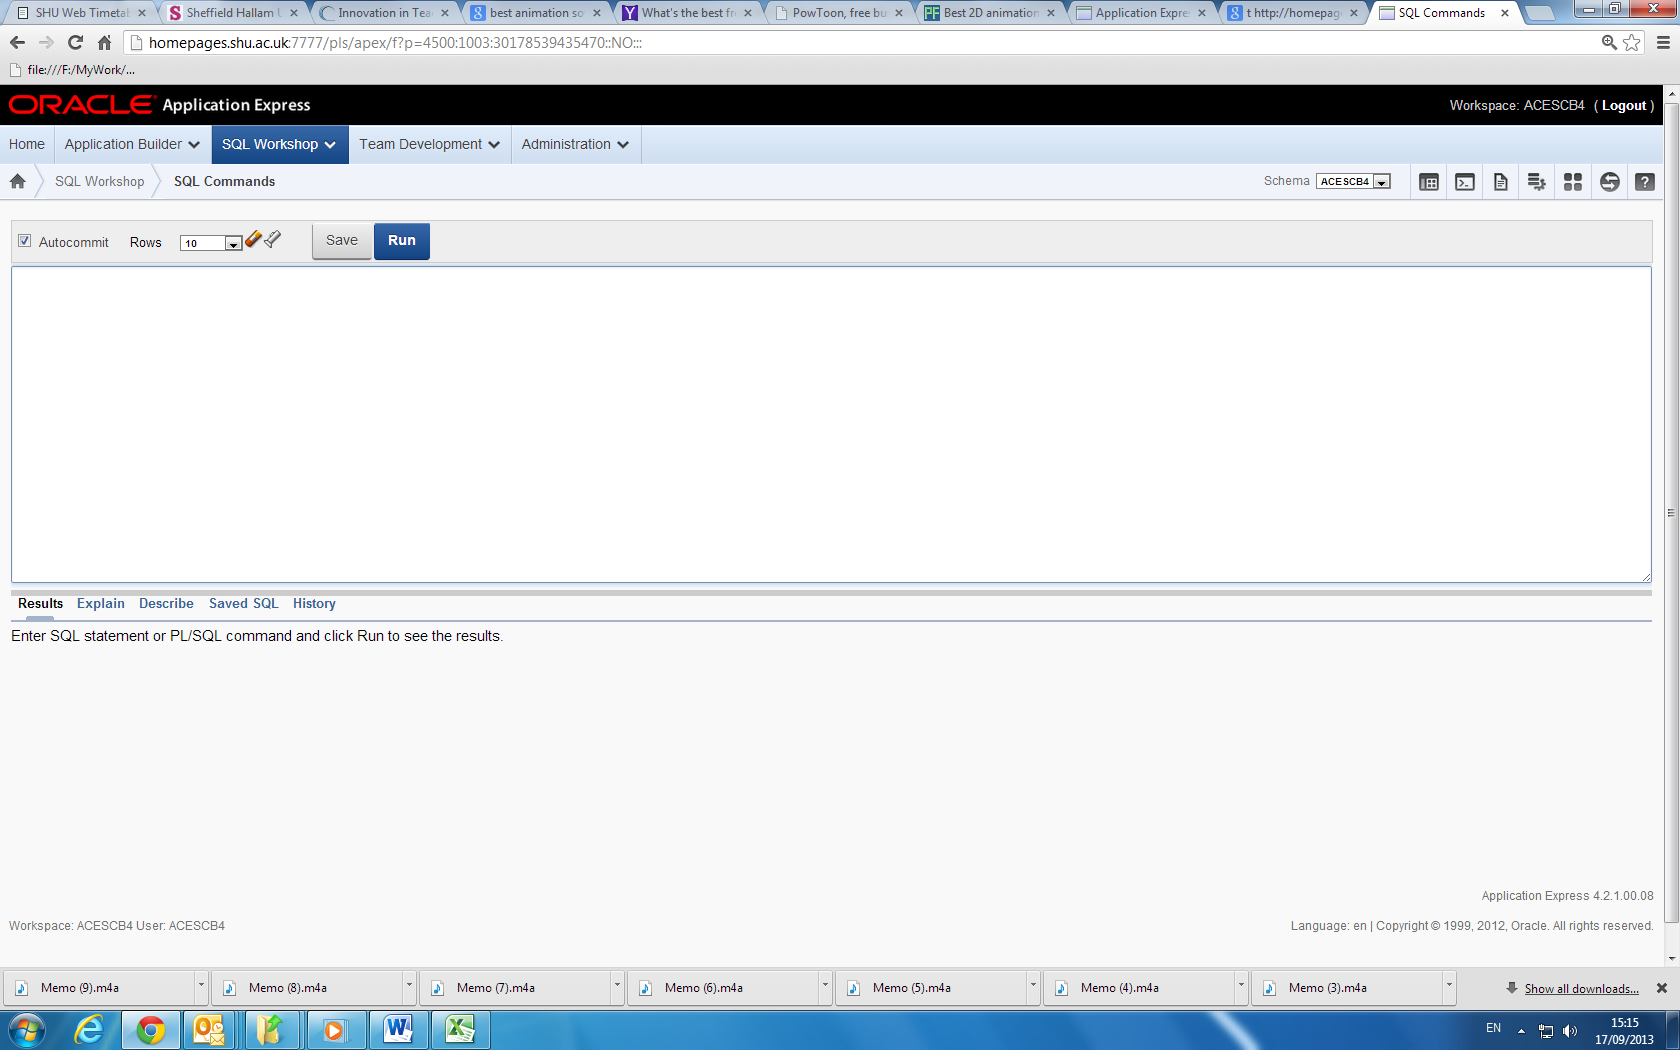
\includegraphics[width=0.947cm,height=0.607cm]{images/img (9).png}
 

and (you don't have to retype, edit the previous command):

Select  *  from EmP; 
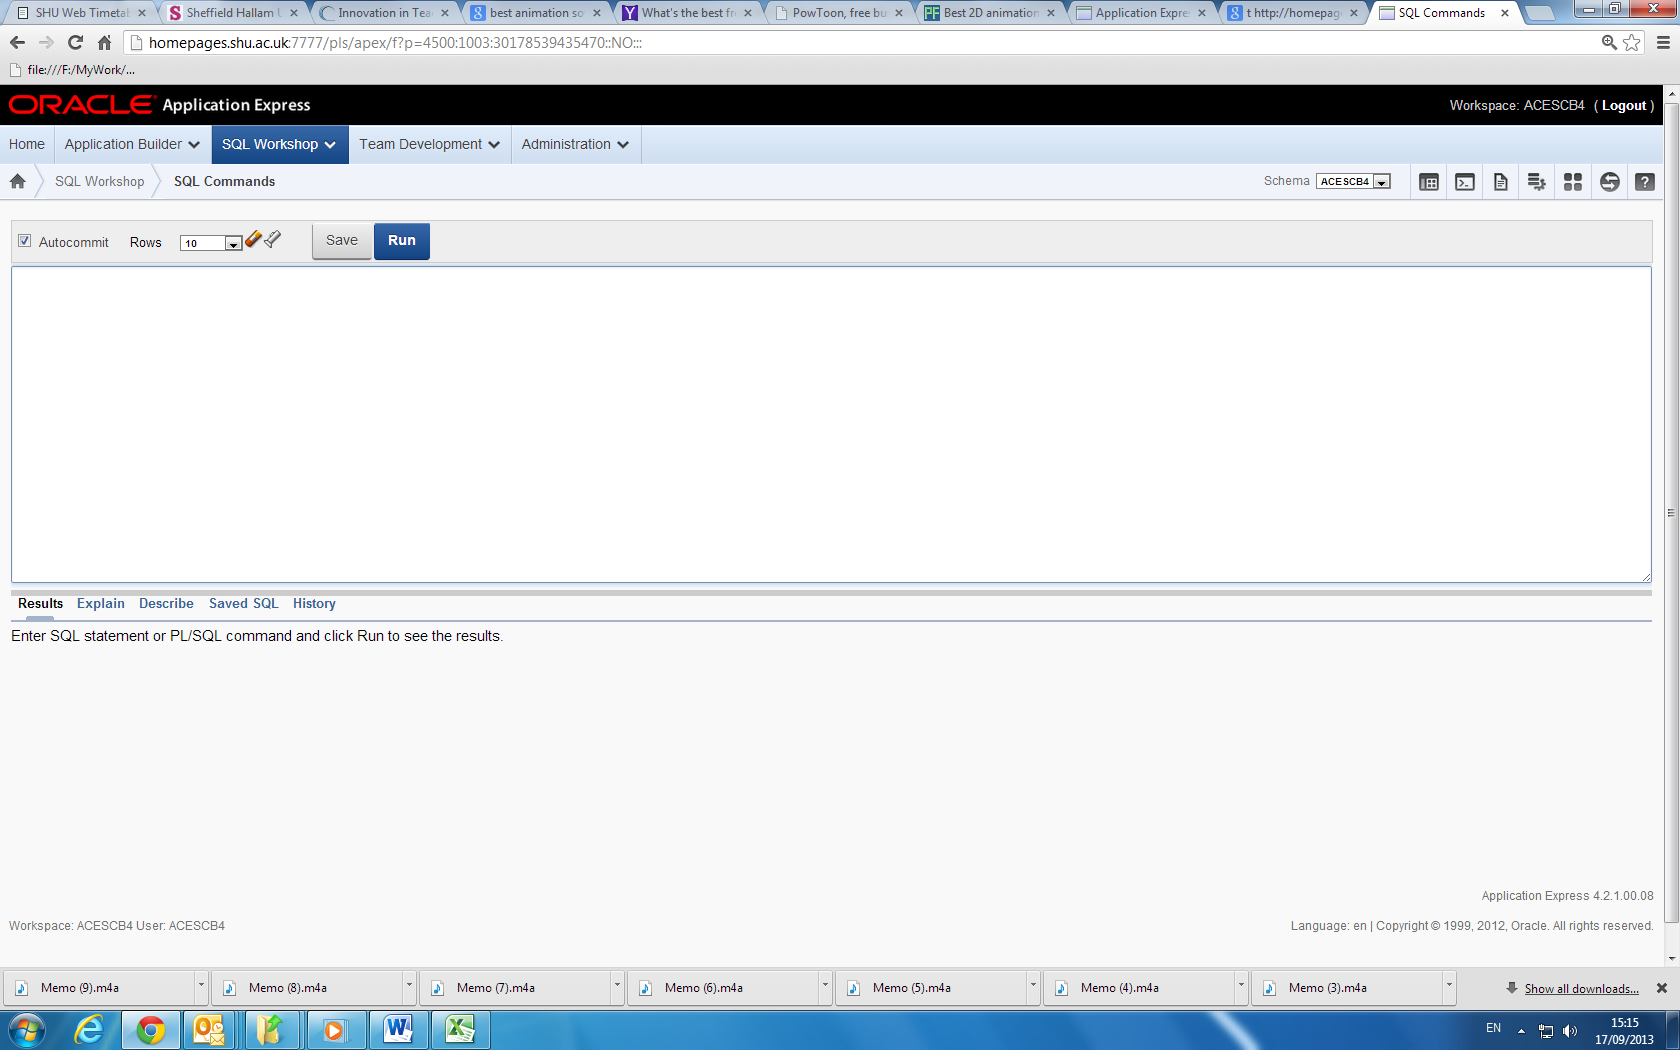
\includegraphics[width=0.947cm,height=0.607cm]{images/img (9).png}
 

Is white space -- new lines, spaces -- allowed in commands? Try

select  *  from  
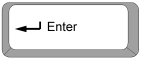
\includegraphics[width=1.63cm,height=0.683cm]{images/img (8).png}
 

 emp; 
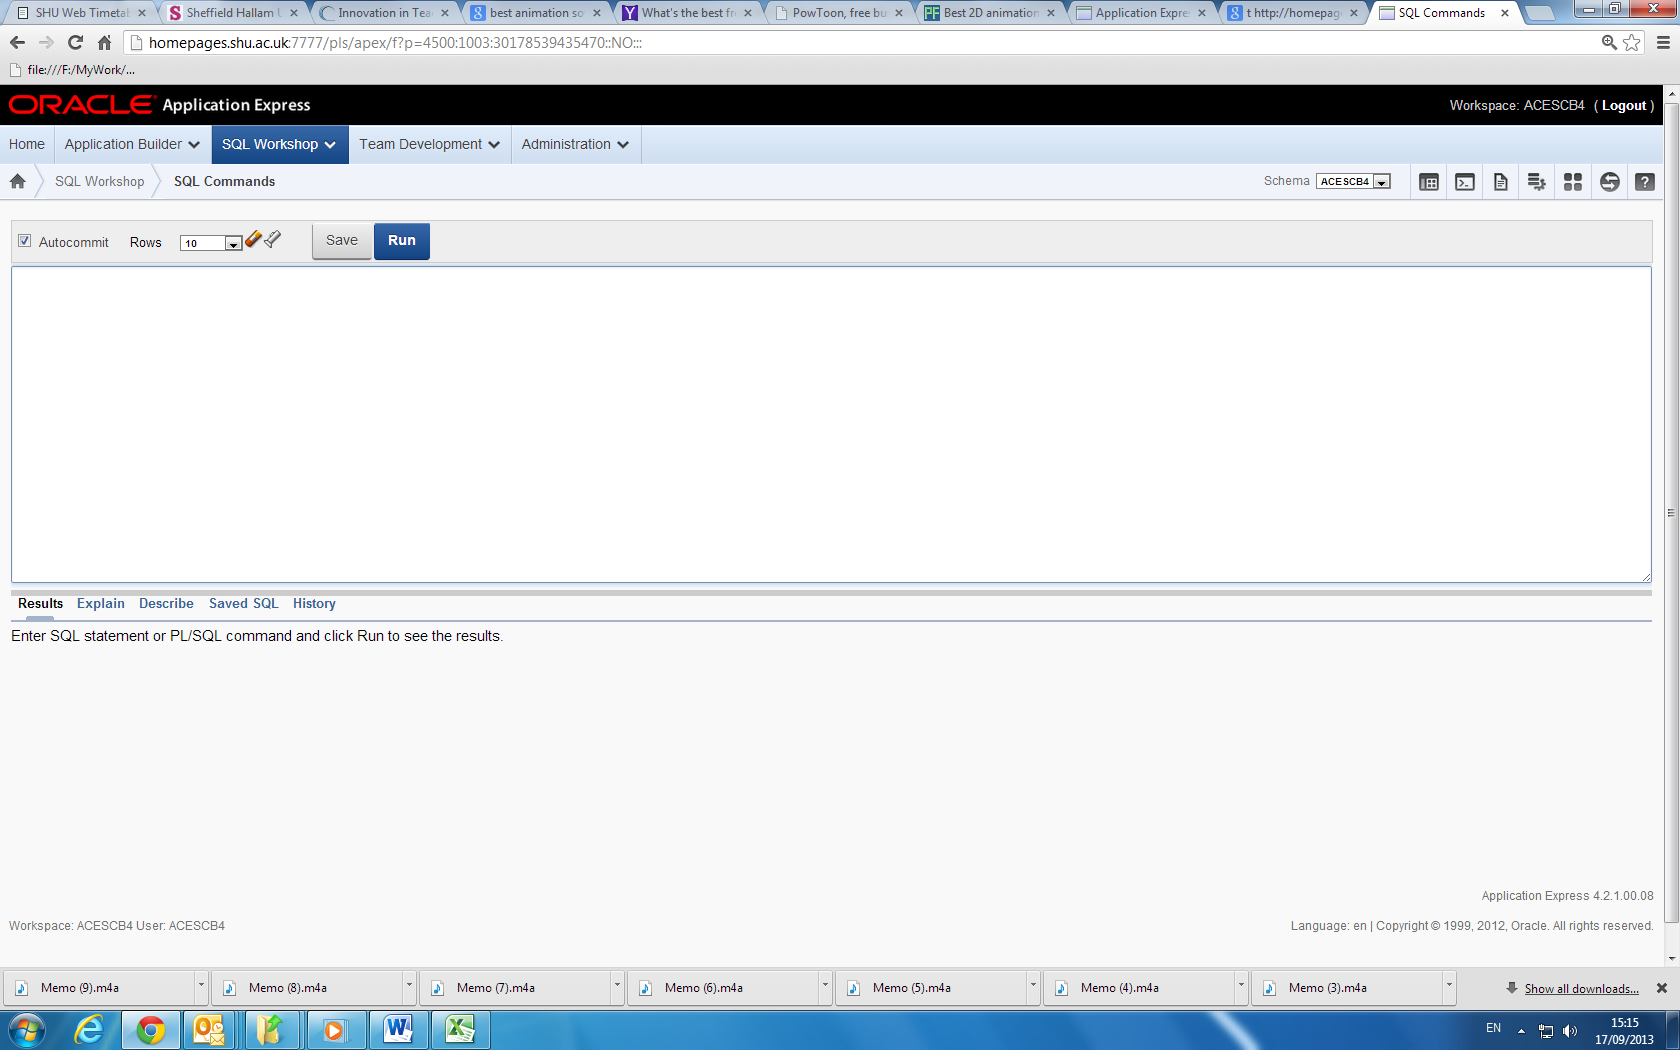
\includegraphics[width=0.947cm,height=0.607cm]{images/img (9).png}
 

You may wish to discuss your conclusions with a colleague. Keep notes of what you find out - about the use of case, of white space, any errors you have to deal with and how you resolve them.



\begin{center}
  

\includegraphics[width=1.048cm,height=0.903cm]{images/img (2).png}

\end{center}
Scribbling on this workbook is definitely allowed!

Oracle techniques

Note: the techniques that follow are ORACLE-specific, and wouldn't work as such with other DB management systems.

Now enter all of the following before pressing the Run button:

\ \ select * from emp;  
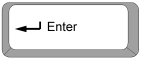
\includegraphics[width=1.63cm,height=0.683cm]{images/img (8).png}
 

\ \ select * from dept;

\begin{center}
  
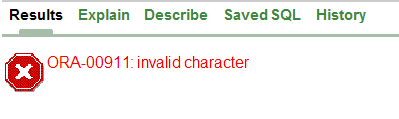
\includegraphics[width=10.137cm,height=3.044cm]{images/img (11).png}

\end{center}
You now have an error message.  Unfortunately the message is unhelpful. SQL statements are correctly separated with a ; (semi-colon), but  from the SQL workshop, Oracle cannot run both statements in succession. One solution is to first highlight the statement you wish to run:

Highlight the first 'select * from emp;' and press the run button.  You should recognise the results.

\section{Checking the objects available}


\begin{center}
  
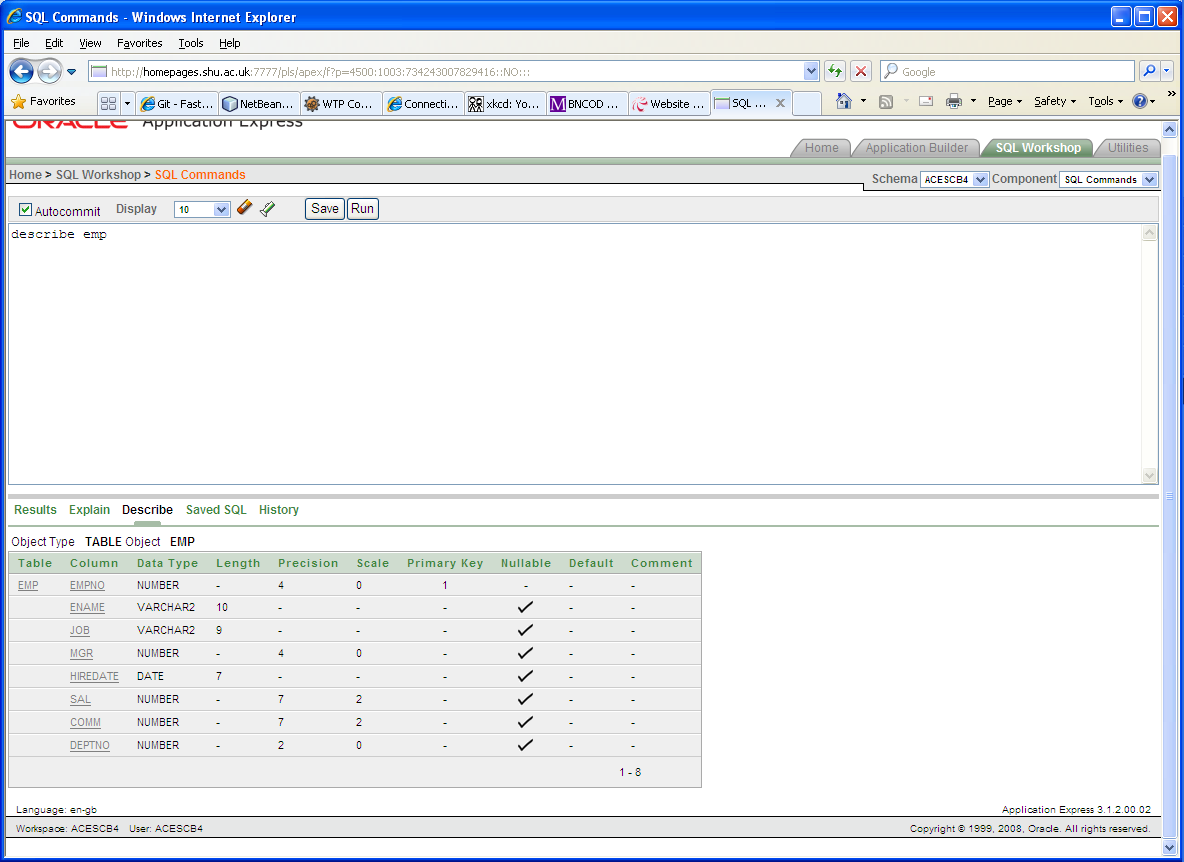
\includegraphics[width=9.35cm,height=4.944cm]{images/img (12).png}

\end{center}
Try this:

\emph{DESCRIBE table\_name;}

is a useful command. It displays a table definition, e.g.

\ \ DESCRIBE\ \ EMP;

gives the result on the right.



\begin{center}
  
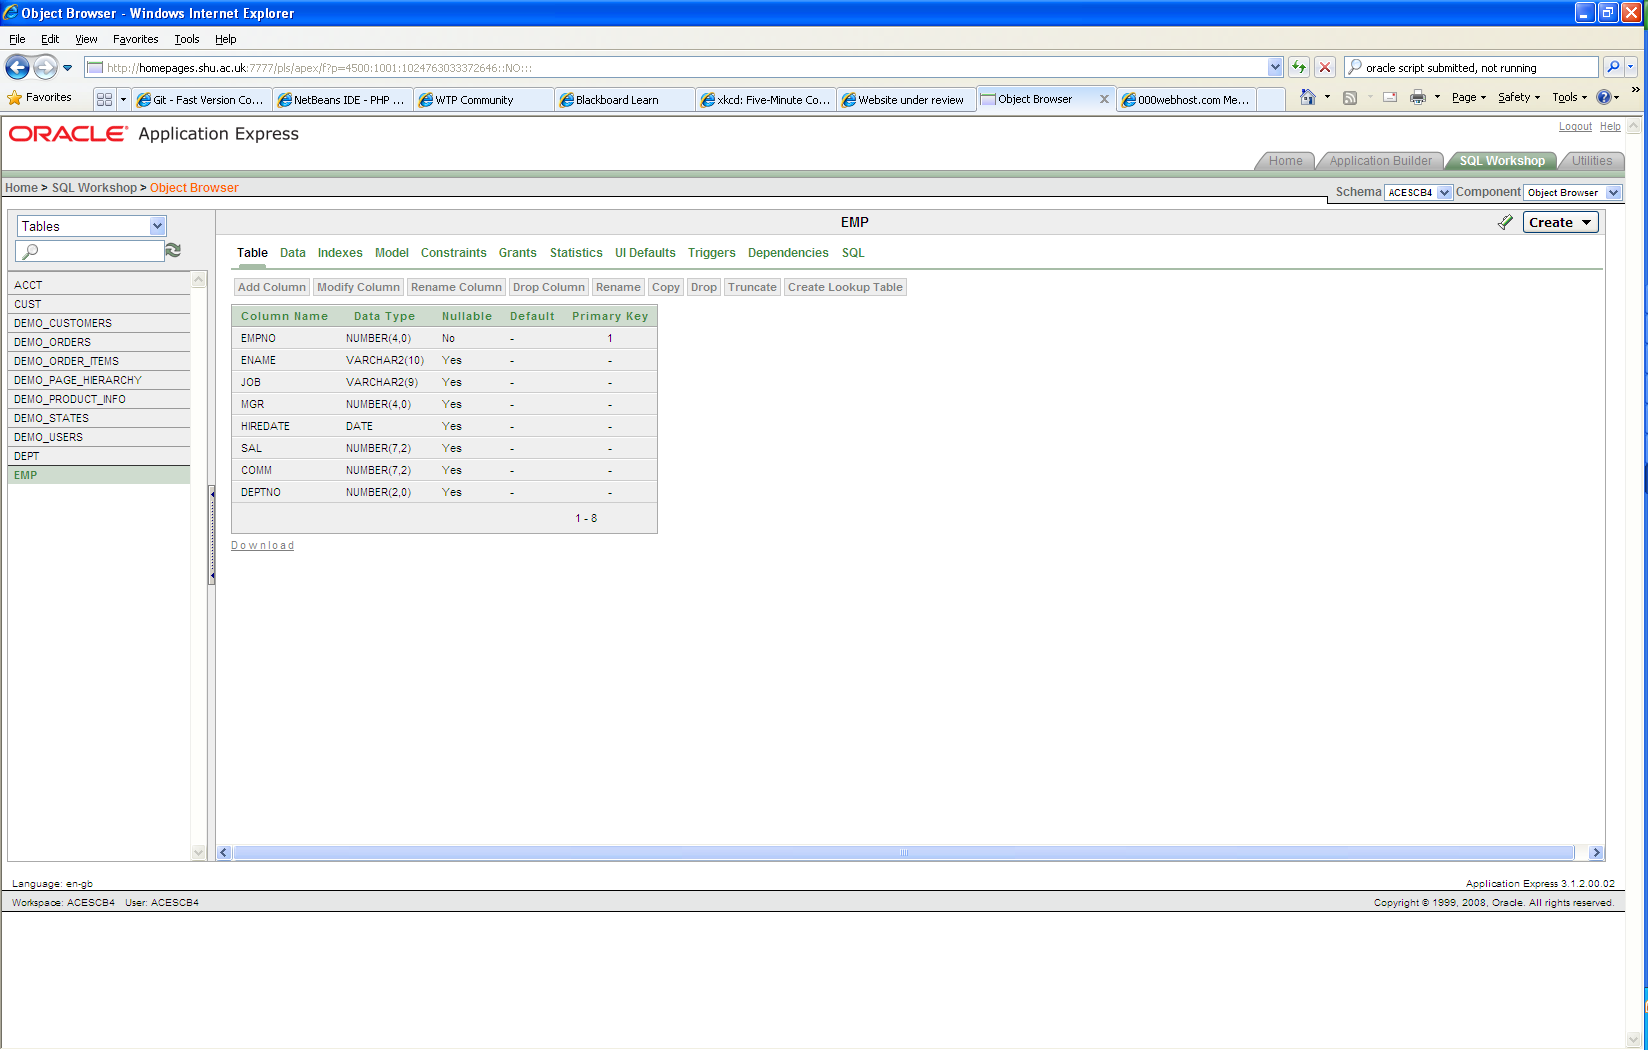
\includegraphics[width=8.751cm,height=5.309cm]{images/img (13).png}

\end{center}
Now move to the 'Home{\textgreater}SQL Workshop' screen and select the 'Object browser' feature. It shows details of all the tables, views and other objects that exist within your Oracle environment. 

Finally, the following gives details of the tables and views you currently own:

SELECT  *  from TAB;

ORACLE has a data dictionary that holds details of the database definition and its environment.  The query returns those details, as if {\textquotedbl}TAB{\textquotedbl} was a table of your tables.

About the exercises

\begin{itemize}
\item Do not rush; take time to understand what is happening.
\item When you get errors, study your statement(s) and the data (or error messages!) to determine a solution; do NOT get into a 'hacking' mode.
\item Think what results you would expect from the statement(s) you are issuing and carefully check them against the generated result.
\item Note your solutions. You can use this workbook for the purpose, or save scripts (one script for each section of the workbook?).  You will find it useful to refer back to earlier work.
\item Discuss problems and uncertainties with your tutor, they are there to help.
\item Maintain progress. Each section is very dependent on understanding previous ones.
\end{itemize}
We hope you enjoy the experience.

\section{About notation to describe SQL syntax}
SQL statements are made of multiple clauses. As they are sometimes difficult to explain, this book describes the different combinations of keywords using some special characters.

\begin{itemize}
\item Anything that needs to be replace is in italics; example:
\end{itemize}
\ \ SELECT * FROM table

table is actually not the word to type, but a word to substitute replace by the name of the actual table you want.

\begin{itemize}
\item Optional elements are included in [square brackets] [ ], are optional. Ffor example:
\end{itemize}
\ \   \ \ SELECT * FROM table [ WHERE Criteria ] ;

cWhich indicates that the section {}``WHERE Criteria{}'' is ould be either:\ \ SELECT * FROM table ;

\ \ or\ \ \ \ \ \ SELECT * FROM table WHERE Criteria ;



\begin{center}
  

\includegraphics[width=1.048cm,height=0.903cm]{images/img (2).png}

\end{center}
in option.

Don't type the square brackets! The same is true of the other signs below the other notation signs below.

\begin{itemize}
\item Optional repetition is marked using ... as follows:
\end{itemize}
\ \   SELECT col1 [ , col2 ... ]  FROM table  [ WHERE Criteria ] ;

This means that there can be one or more columns.

\begin{itemize}
\item Finally, we use and the vertical bar {\textbar} (also called the pipe symbol) and if need be, braces \{ \} to denote alternatives:
\end{itemize}
 SELECT \{ * {\textbar} columns-list \} FROM table ;

Means that you can use either a list of columns, or the * with this statement.

\clearpage

\chapter{the SELECT statement: Extracting Data}
The SELECT statement is used to retrieve and display data from one or more tables.  The constructs in this section have the general form:

\ \   SELECT [ DISTINCT ]\ \ desired columns

\ \   FROM\ \ table

\ \ [ WHERE\ \ criteria for rows ]

\ \ [ ORDER BY\ \ Sorting sequence ]

\ \   ;

Only the first two clauses SELECT ... and FROM ... and the terminating  ;  are mandatory.



\begin{center}
  

\includegraphics[width=1.048cm,height=0.903cm]{images/img (2).png}

\end{center}
\begin{center}
\begin{minipage}{4.849cm}
   

\includegraphics[width=4.553cm,height=4.553cm]{images/img (14).png}
 

   

\includegraphics[width=1.582cm,height=0.674cm]{images/img (15).png}
 
\end{minipage}
\end{center}
Remember - anything in [brackets] is in option.

 (anything in [ ] is optional)

Selecting all the data from a single table: -

\ \ SELECT  *  FROM  table-name;

This will display all columns, ffor example:

\ \ SELECT \ \  * 

\ \  FROM \ \ \ \  EMP;

Displays all columns from the EMP table:

   
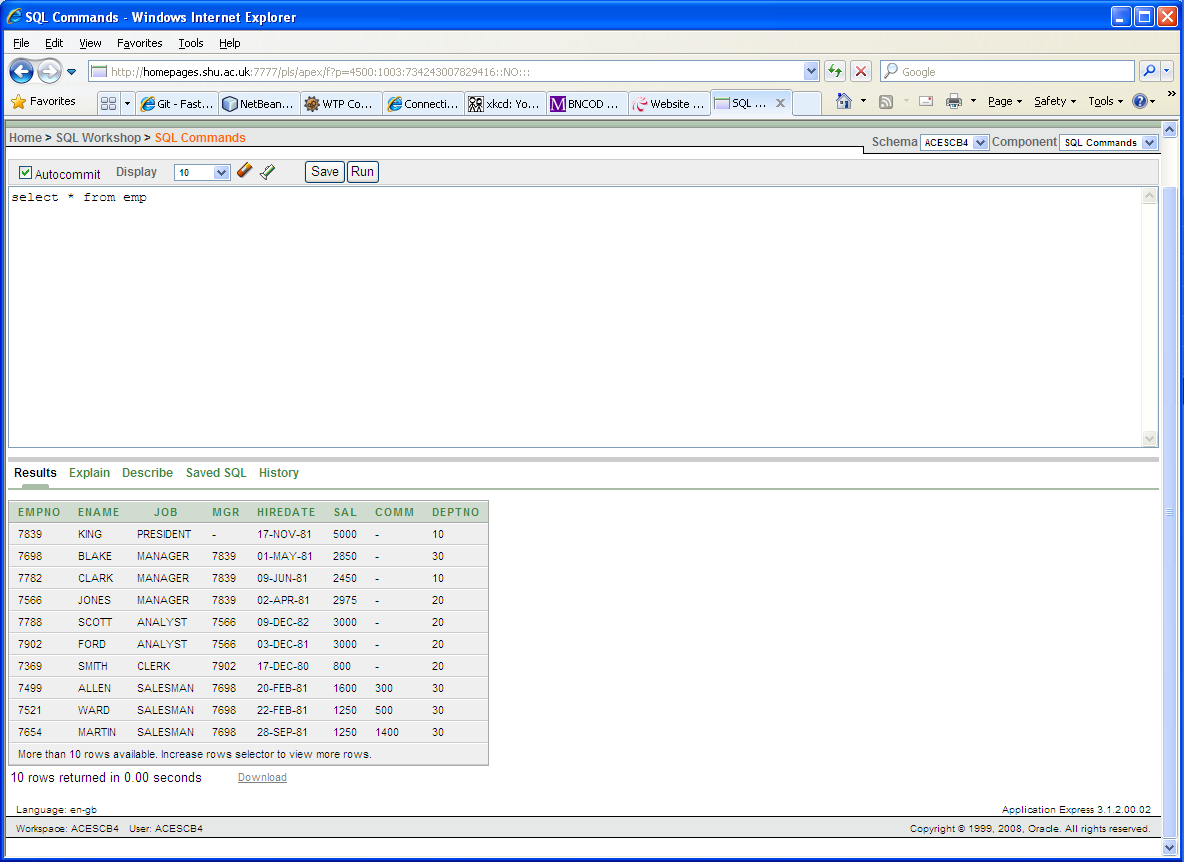
\includegraphics[width=14.785cm,height=7.089cm]{images/img (10).png}
 

The rows show in the same order as they were entered.

B1\ \ Display all the contents of the DEPT, EMP and SALGRADE tables.

\begin{flushleft}
\tablefirsthead{}
\tablehead{}
\tabletail{}
\tablelasttail{}
\begin{supertabular}{|m{14.405cm}|}
\hline
Select * from EMP ;\\\hline
Select\\\hline
Select\\\hline
\end{supertabular}
\end{flushleft}
To identify all your tables and views, use the special table, TAB

\ \ SELECT\ \ \ \  *

\ \ FROM\ \ \ \ \ \  TAB ;



\begin{center}
  
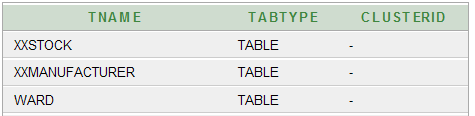
\includegraphics[width=12.298cm,height=2.992cm]{images/img (16).png}

\end{center}
To control which columns are displayed, and the order of them;-

\ \ SELECT  col1 [ , col2 ... ] FROM table-name;

Displays named columns.



\begin{center}
  

\includegraphics[width=1.076cm,height=0.917cm]{images/img (2).png}

\end{center}
There is a comma between each column name, but not after the final one.

For example, here are all employees with their employee number, name \& department number:

\ \ SELECT\ \ EmpNo,

\begin{center}
  
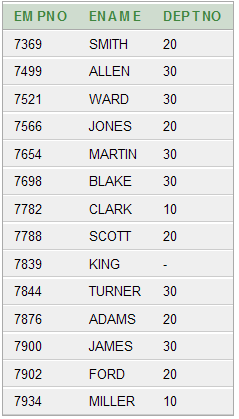
\includegraphics[width=5.826cm,height=5.6cm]{images/img (17).png}

\end{center}
\ \ \ \ \ \ Ename,

\ \ \ \ \ \ DeptNo

\begin{center}
  
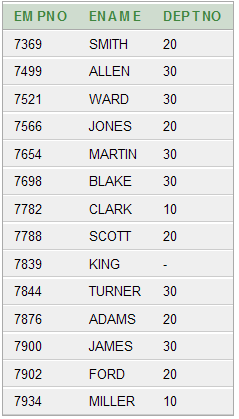
\includegraphics[width=5.826cm,height=4.662cm]{images/img (17).png}

\end{center}
\ \ FROM\ \ \ \ Emp ;

Below, REFNO NAME will would be displayed before NAME REFNO even though the table was first setup y were initially defined the other way round.  



\begin{center}
\begin{minipage}{5.191cm}
\begin{flushleft}
\tablefirsthead{}
\tablehead{}
\tabletail{}
\tablelasttail{}
\begin{supertabular}{|m{2.2389998cm}|m{2.55cm}|}
\hline
REFNO &
NAME\\\hline
A123 &
J Doe\\
A124 &
J Smith\\
B127 &
R Best\\
B128 &
J Best\\
C371 &
R Done\\\hline
\end{supertabular}
\end{flushleft}
\end{minipage}
\end{center}
SELECT\ \ REFNO,

\ \ \ \ NAME 

FROM\ \ \ \ \ \ \ \ CUST ;

For all the following exercises record the statement that will give you the required output.  Check against the given tables to ensure that the correct rows are selected and save the statements for future reference. 

(For each section the output from some of the queries is reproduced for you, but after that you are on your own!)

B2\ \ Display the name and commission of all the employees.



\begin{center}
  
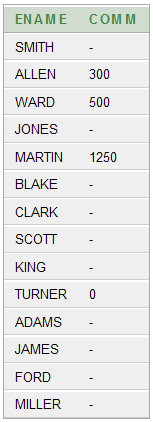
\includegraphics[width=3.281cm,height=4.748cm]{images/img (18).png}

\end{center}
\begin{center}
  
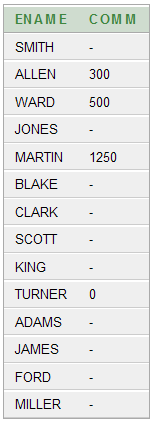
\includegraphics[width=3.27cm,height=4.12cm]{images/img (19).png}

\end{center}
\begin{flushleft}
\tablefirsthead{}
\tablehead{}
\tabletail{}
\tablelasttail{}
\begin{supertabular}{|m{7.051cm}|}
\hline
Select 

\\\hline
\end{supertabular}
\end{flushleft}

B3\ \ Display the job title of all the employees.

\begin{center}
  
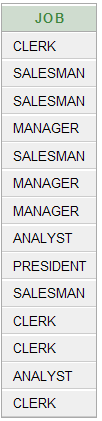
\includegraphics[width=2.42cm,height=4.623cm]{images/img (20).png}

\end{center}
\begin{center}
  
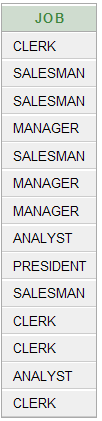
\includegraphics[width=2.431cm,height=5.398cm]{images/img (20).png}

\end{center}
\begin{flushleft}
\tablefirsthead{}
\tablehead{}
\tabletail{}
\tablelasttail{}
\begin{supertabular}{|m{8.0cm}|}
\hline
Select 

\\\hline
\end{supertabular}
\end{flushleft}
\section{Using DISTINCT}
It is not good practice to repeat values as part of the answer to such a question.  To remove duplicates within the result table, use the distinct keyword:

\ \ SELECT DISTINCT col1 [ , col2 ... ]  FROM  table-name ;

B4\ \ Display all the different job titles which currently exist in the company.

\begin{center}
  
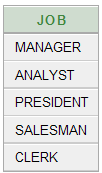
\includegraphics[width=2.491cm,height=4.124cm]{images/img (21).png}

\end{center}
\begin{flushleft}
\tablefirsthead{}
\tablehead{}
\tabletail{}
\tablelasttail{}
\begin{supertabular}{|m{11.537001cm}|}
\hline
Select 

\\\hline
\end{supertabular}
\end{flushleft}
\section{Simple calculations and column aliases}
It is also possible to manipulate the column values before displaying them: -



\begin{center}
\begin{minipage}{4.849cm}
   

\includegraphics[width=4.314cm,height=4.314cm]{images/img (22).png}
 

   

\includegraphics[width=1.582cm,height=0.674cm]{images/img (15).png}
 
\end{minipage}
\end{center}
\ \ SELECT\ \ col1 ,

\ \ \ \ \ \ col2*2.5 ,

\ \ \ \ \ \ col3+col4 AS alias1  {}-{}-  etc. note the column-renaming

\ \ FROM\ \ \ \ table-name ;

this displays specified columns, performs arithmetic on columns, and specifies an alias name to use as a column heading for the output.

For example, this:

SELECT\ \ ACCNO, BALANCE,

\begin{center}
\begin{minipage}{6.943cm}
\begin{flushright}
\tablefirsthead{}
\tablehead{}
\tabletail{}
\tablelasttail{}
\begin{supertabular}{|m{1.9909999cm}|m{2.299cm}|m{2.052cm}|}
\hline
ACCNO &
BALANCE &
BONUS\\\hline
1245890 &
\raggedleft 234.50 &
\raggedleft\arraybslash 23.45\\
1494315 &
\raggedleft 0.50 &
\raggedleft\arraybslash 0.05\\
5418490 &
\raggedleft 1789.40 &
\raggedleft\arraybslash 178.94\\\hline
\end{supertabular}
\end{flushright}
\end{minipage}
\end{center}
\ \ BALANCE * 0.1  AS BONUS

FROM\ \ ACC ;

Wouldill produce the result shown on the right.

B5\ \ Display the name and commission of all the employees together with another column that shows their commission increased by 10\%.  Use an appropriate column alias for the new column.



\begin{center}
  
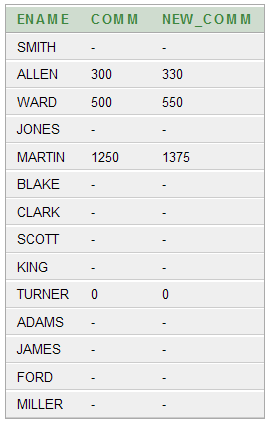
\includegraphics[width=7.17cm,height=6.218cm]{images/img (23).png}

\end{center}
\begin{flushleft}
\tablefirsthead{}
\tablehead{}
\tabletail{}
\tablelasttail{}
\begin{supertabular}{|m{6.8570004cm}|}
\hline
Select 

\\\hline
\end{supertabular}
\end{flushleft}
\section{The WHERE clause}
To SELECT specific rows from a single table the optional WHERE clause is used, for example:  Display all the customers in the Sheffield area:

\ \ SELECT *

\begin{center}
\begin{minipage}{9.192cm}
\begin{flushleft}
\tablefirsthead{}
\tablehead{}
\tabletail{}
\tablelasttail{}
\begin{supertabular}{|m{1.742cm}|m{1.798cm}|m{2.8cm}|m{2.049cm}|}
\hline
REFNO &
NAME &
ADDRESS &
AREA\\\hline
A123 &
J Doe &
1 High Street &
Sheffield\\
A124 &
J Smith &
2 West Street &
Sheffield\\
\end{supertabular}
\end{flushleft}
\end{minipage}
\end{center}
\ \ FROM CUST 

\ \ WHERE AREA = 'Sheffield' ;

WHERE is followed by an expression that will be either true or false (a Boolean). The simpler ones look like:

\begin{center}
\begin{minipage}{4.849cm}
   

\includegraphics[width=4.314cm,height=4.314cm]{images/img (24).png}
 

   

\includegraphics[width=1.582cm,height=0.674cm]{images/img (15).png}
 
\end{minipage}
\end{center}
Column  = Value

Value will be in quotes for text, but not for numbers, e.g.

AREA = 'Sheffield'

or

DEPTNO = 30

B6\ \ Display the employee number, name and current job of all those who work in Department 30.

\begin{center}
  
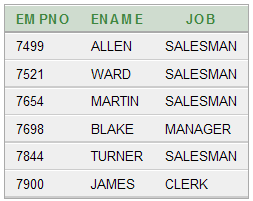
\includegraphics[width=4.9cm,height=3.861cm]{images/img (25).png}

\end{center}
\begin{flushleft}
\tablefirsthead{}
\tablehead{}
\tabletail{}
\tablelasttail{}
\begin{supertabular}{|m{9.202001cm}|}
\hline
Select 

From

Where\\\hline
\end{supertabular}
\end{flushleft}
B7\ \ Display the names of all the clerks, showing their employee number and that of their manager.  Note: strings are case sensitive and in single quote marks.

\begin{flushleft}
\tablefirsthead{}
\tablehead{}
\tabletail{}
\tablelasttail{}
\begin{supertabular}{|m{14.303cm}|}
\hline
Select 

\\\hline
\end{supertabular}
\end{flushleft}
\emph{As well as = other comparison operators are allowed: {\textless} ; {\textless}= ; {\textgreater} ;  {\textgreater}= ; {\textless}{\textgreater} and !=}

(!= and {\textless}{\textgreater} both mean not equal; do you know all the others?)

B8\ \ Display details of all employees whose commission is greater than salary.

\begin{flushleft}
\tablefirsthead{}
\tablehead{}
\tabletail{}
\tablelasttail{}
\begin{supertabular}{|m{14.303cm}|}
\hline
Select 

\\\hline
\end{supertabular}
\end{flushleft}
We can also use calculations involving columns in the comparisons, just as we do to display calculations

B9\ \ Display name, a twentieth of salary as 'Twentieth' and commission of all employees whose commission is greater than a twentieth of their salary.

\begin{flushleft}
\tablefirsthead{}
\tablehead{}
\tabletail{}
\tablelasttail{}
\begin{supertabular}{|m{14.303cm}|}
\hline
Select 

\\\hline
\end{supertabular}
\end{flushleft}
True or false expressions can be combined with logical operators AND, OR:

WHERE Exp1 OR Exp2

WHERE Exp1 AND Exp2



\begin{center}
  

\includegraphics[width=1.06cm,height=0.903cm]{images/img (2).png}

\end{center}
The AND and OR operators combine Boolean expression together. So this doesn't work:



\begin{center}
  

\includegraphics[width=1.443cm,height=1.427cm]{images/img (26).png}

\end{center}
SELECT  *

FROM  emp

WHERE deptno = 30 OR 40;

These do:

SELECT  *

\begin{center}
  

\includegraphics[width=1.443cm,height=1.184cm]{images/img (27).png}

\end{center}
FROM  emp

WHERE deptno = 30 OR deptno = 40;

SELECT  *

\begin{center}
  

\includegraphics[width=1.443cm,height=1.184cm]{images/img (27).png}

\end{center}
FROM  emp

WHERE deptno = 30 AND job = `MANAGER';

B10\ \ Display details of all clerks and analysts.  

\begin{flushleft}
\tablefirsthead{}
\tablehead{}
\tabletail{}
\tablelasttail{}
\begin{supertabular}{|m{14.303cm}|}
\hline
Select 

\\\hline
\end{supertabular}
\end{flushleft}
B11\ \ Display details of all clerks, analysts and salesmen.

\begin{flushleft}
\tablefirsthead{}
\tablehead{}
\tabletail{}
\tablelasttail{}
\begin{supertabular}{|m{14.303cm}|}
\hline
Select 

\\\hline
\end{supertabular}
\end{flushleft}
The operator NOT can be used in front of a Boolean:

WHERE NOT Exp;



\begin{center}
  

\includegraphics[width=1.06cm,height=0.903cm]{images/img (2).png}

\end{center}
The NOT operator is placed in front of a Boolean expression. So this doesn't work:



\begin{center}
  

\includegraphics[width=1.443cm,height=1.427cm]{images/img (26).png}

\end{center}
SELECT  *

FROM  emp

WHERE deptno = NOT 30;

These do:

SELECT  *

\begin{center}
  

\includegraphics[width=1.443cm,height=1.184cm]{images/img (27).png}

\end{center}
FROM  emp

WHERE NOT deptno = 30;

SELECT  *

\begin{center}
  

\includegraphics[width=1.443cm,height=1.184cm]{images/img (27).png}

\end{center}
FROM  emp

WHERE deptno != 30;

\ \ \ \ \ \ \ \ Remember that != is the 'not equal' operator 

B12\ \ Display details of employees who are neither managers nor president; you must not use knowledge about other jobs that might exist.

\begin{flushleft}
\tablefirsthead{}
\tablehead{}
\tabletail{}
\tablelasttail{}
\begin{supertabular}{|m{14.303cm}|}
\hline
Select 

\\\hline
\end{supertabular}
\end{flushleft}
There are several more useful construct and operators for Boolean expressions:

WHERE Value1 [ NOT ] BETWEEN Value2 AND Value3

WHERE Value  [ NOT ] IN (Value1 [ , Value2 , ... ] )

WHERE Value   [ NOT ] LIKE '\%charstring\%{}'

(\% means skip 0 to n characters) 

WHERE Value  [ NOT ] LIKE 'string1\_string2{}'

( \_ means for one and only one character)

WHERE Value IS [ NOT ] NULL

(The action of the BETWEEN, IN, LIKE and IS operators can be negated by NOT. Note that in these the case of constructs{}'IS NOT NULL', exceptionally, you can position the NOT operator as you would in English, rather than in front of the expression ).



\begin{center}
  
\includegraphics[width=1.06cm,height=0.903cm]{images/img (2).png}

\end{center}
To understand the constructs above takes more than this book. Refer to other material -- e.g. lectures - to work it out.

B13\ \ Display employee name, job and department number for employees whose names begin with `M'.

\begin{center}
\begin{minipage}{4.849cm}
   
\includegraphics[width=4.341cm,height=4.341cm]{images/img (28).png}
 

   
\includegraphics[width=1.582cm,height=0.674cm]{images/img (15).png}
 
\end{minipage}
\end{center}
\begin{flushleft}
\tablefirsthead{}
\tablehead{}
\tabletail{}
\tablelasttail{}
\begin{supertabular}{|m{11.493cm}|}
\hline
 Select 

\\\hline
\end{supertabular}
\end{flushleft}
B14\ \ Find a second way of answering B11 (details of all clerks, analysts and salesmen). Your solution must not use knowledge about other jobs that might exist.

\begin{flushleft}
\tablefirsthead{}
\tablehead{}
\tabletail{}
\tablelasttail{}
\begin{supertabular}{|m{12.782001cm}|}
\hline
Select 

\\\hline
\end{supertabular}
\end{flushleft}
B15\ \ Find a second way of answering B12 (employees who are neither managers nor president); again you must not use knowledge about other jobs that might exist. 

\begin{flushleft}
\tablefirsthead{}
\tablehead{}
\tabletail{}
\tablelasttail{}
\begin{supertabular}{|m{14.368cm}|}
\hline
Select 

\\\hline
\end{supertabular}
\end{flushleft}
B16\ \ Display details of employees who are not clerks, analysts or salesmen.  Write two different instructions to achieve this.

\begin{flushleft}
\tablefirsthead{}
\tablehead{}
\tabletail{}
\tablelasttail{}
\begin{supertabular}{|m{14.303cm}|}
\hline
Select 

\\\hline
Select 

\\\hline
\end{supertabular}
\end{flushleft}
B17\ \ Display details of employees whose salaries are between £1,200 and £1,400.  Write two different instructions to achieve this.

\begin{flushleft}
\tablefirsthead{}
\tablehead{}
\tabletail{}
\tablelasttail{}
\begin{supertabular}{|m{14.303cm}|}
\hline
Select 

\\\hline
Select 

\\\hline
\end{supertabular}
\end{flushleft}
B18\ \ Display details of employees whose salaries are not between £1,200 and £1,400.  Write two different instructions to achieve this.  Ensure you check your results!

\begin{flushleft}
\tablefirsthead{}
\tablehead{}
\tabletail{}
\tablelasttail{}
\begin{supertabular}{|m{14.303cm}|}
\hline
Select 

\\\hline
Select 

\\\hline
\end{supertabular}
\end{flushleft}
B19\ \ Display details of those salesmen and managers in dept 30 whose salary is greater than or equal to £1,500.  Check your results carefully.

\ \ \ \ (Note: for logical operators - AND takes precedence over OR).

Complex instructions may be written and tested in stages, building the complexity with each step.

Stage 1: Display details of salesmen and managers.

\begin{flushleft}
\tablefirsthead{}
\tablehead{}
\tabletail{}
\tablelasttail{}
\begin{supertabular}{|m{14.303cm}|}
\hline
Select 

\\\hline
\end{supertabular}
\end{flushleft}
Stage 2: Display details of those salesmen and managers in Department 30.  Run the instruction and check your results.

\begin{flushleft}
\tablefirsthead{}
\tablehead{}
\tabletail{}
\tablelasttail{}
\begin{supertabular}{|m{14.303cm}|}
\hline
Select 

\\\hline
\end{supertabular}
\end{flushleft}
Stage 3: Display details of those salesmen and managers in dept 30 whose salary is greater than or equal to £1,500.  Check your results carefully.

\begin{flushleft}
\tablefirsthead{}
\tablehead{}
\tabletail{}
\tablelasttail{}
\begin{supertabular}{|m{14.303cm}|}
\hline
Select 

\\\hline
\end{supertabular}
\end{flushleft}
\section[The ORDER BY clause]{The ORDER BY clause}
The ORDER BY clause is used to control the display order of selected records

ORDER BY\ \ col1 [ , col2 ... ]\ \ \ \ (first by col1, then by col2, etc.)

ORDER BY\ \ col1  [ ASC {\textbar} DESC ]\ \ (by col1, ascending, or descending)

ORDER BY \ \ n ; \ \ \ \ \ \ \ \ (by the nth column)



\begin{center}
  
\includegraphics[width=1.076cm,height=0.917cm]{images/img (2).png}

\end{center}
Note: The default ordering is ascending.

Null values are always displayed first regardless of sort sequence.

B20\ \ Display the employee number, current job and salary of all those who work in Department 30, with the output in ascending salary order.  As before, you may wish to write and test your instruction in a number of stages.



\begin{center}
  
\includegraphics[width=5.514cm,height=4.835cm]{images/img (29).png}

\end{center}
\begin{flushleft}
\tablefirsthead{}
\tablehead{}
\tabletail{}
\tablelasttail{}
\begin{supertabular}{|m{9.482cm}|}
\hline
Select 

From

Where

Order By\\\hline
\end{supertabular}
\end{flushleft}


\begin{center}
\begin{minipage}{4.849cm}
   
\includegraphics[width=4.314cm,height=4.314cm]{images/img (22).png}
 

   
\includegraphics[width=1.582cm,height=0.674cm]{images/img (15).png}
 
\end{minipage}
\end{center}
B21\ \ Display the employee name and current job of all those who work in Department 30, with the output in descending salary order.

\begin{flushleft}
\tablefirsthead{}
\tablehead{}
\tabletail{}
\tablelasttail{}
\begin{supertabular}{|m{9.644cm}|}
\hline
Select 

\\\hline
\end{supertabular}
\end{flushleft}
Note: \ \ You were asked to order the rows using a column that is not selected for display; maybe a little unusual but not impossible.  How have you checked the accuracy of your result?

\begin{center}
  
\includegraphics[width=1.06cm,height=0.903cm]{images/img (2).png}

\end{center}
B22\ \ Display employee details for Departments 10 and 30, in name order, within each department.  Display the columns in the most appropriate order.

\begin{flushleft}
\tablefirsthead{}
\tablehead{}
\tabletail{}
\tablelasttail{}
\begin{supertabular}{|m{14.303cm}|}
\hline
Select 

\\\hline
\end{supertabular}
\end{flushleft}
B23\ \ Display the employee name, current job and salary of all those who work in Department 30, with the output in descending salary order within each job.

\begin{flushleft}
\tablefirsthead{}
\tablehead{}
\tabletail{}
\tablelasttail{}
\begin{supertabular}{|m{14.303cm}|}
\hline
Select 

\\\hline
\end{supertabular}
\end{flushleft}
The question asked for the selected data to be output in descending salary order within each job.  Does this influence the best order for displaying the columns?  Check the output of question B23 and suggest a better column order here.

\begin{flushleft}
\tablefirsthead{}
\tablehead{}
\tabletail{}
\tablelasttail{}
\begin{supertabular}{|m{14.303cm}|}
\hline
Select 

\\\hline
\end{supertabular}
\end{flushleft}

\section{Dates}
Within Oracle, dates are stored and may be used just like any other number column.  To match or enter a date the value must be enclosed in single quote marks, dates may be in one of the formats:

\begin{center}
\begin{minipage}{4.849cm}
   
\includegraphics[width=4.341cm,height=4.341cm]{images/img (30).png}
 

   
\includegraphics[width=1.582cm,height=0.674cm]{images/img (15).png}
 
\end{minipage}
\end{center}
\ \ dd-mmm-yyyy  \ \ eg  {}'01-jan-2001'

\ \ dd/mmm/yyyy \ \ eg  {}'01/jan/2001' \ \ 

\ \ dd mmm yyyy \ \ eg  {}'01 jan 2001'

Without formatting, all dates will be displayed in the two-character year format dd-mmm-yy.



\begin{center}
  
\includegraphics[width=1.06cm,height=0.903cm]{images/img (2).png}

\end{center}
Avoid the two character date format: '01-jan-14' could be the year 14, instead of  2014.

B24\ \ Display details of employees recruited before 1st March 1981, in hire date order.  

\begin{flushleft}
\tablefirsthead{}
\tablehead{}
\tabletail{}
\tablelasttail{}
\begin{supertabular}{|m{14.303cm}|}
\hline
Select 

\\\hline
\end{supertabular}
\end{flushleft}
Date values can be compared using the same operators as numbers, and calculated on as if counting the number of days.

B25\ \ Display details of employees who were recruited during 1983.  Do NOT use wildcards.

\begin{flushleft}
\tablefirsthead{}
\tablehead{}
\tabletail{}
\tablelasttail{}
\begin{supertabular}{|m{14.303cm}|}
\hline
Select 

\\\hline
\end{supertabular}
\end{flushleft}
Oracle uses the variable SYSDATE for today's date. You should use this variable as you use column names.

SYSDATE is not, strictly speaking, todays date -- it is the system date on the Oracle server. The server could be in a different time zone, or poorly setup.

\begin{center}
  
\includegraphics[width=1.06cm,height=0.903cm]{images/img (2).png}

\end{center}
B26\ \ Display, in chronological order, the name, hire date and job details of employees who have been with the company for more than approximately 33 years.  Ensure the statement will work equally well today and in a month's time.  Do NOT pre-calculate any values you use. Hint: remember that dates are held and calculated on as a number of days.

\begin{flushleft}
\tablefirsthead{}
\tablehead{}
\tabletail{}
\tablelasttail{}
\begin{supertabular}{|m{14.303cm}|}
\hline
Select 

\\\hline
\end{supertabular}
\end{flushleft}
At times there will be no obvious table involved.  In such situations, Oracle provides the special table DUAL.

To display calculations:

\ \ SELECT 6 * 365 from DUAL ;

Test sysdate:

\ \ SELECT SYSDATE from DUAL ;

Or the current user:

\ \ SELECT USER from DUAL ;

B27\ \ Use Sysdate to display yesterday's date.

\begin{flushleft}
\tablefirsthead{}
\tablehead{}
\tabletail{}
\tablelasttail{}
\begin{supertabular}{|m{14.303cm}|}
\hline
SELECT 

FROM dual;

\\\hline
\end{supertabular}
\end{flushleft}
\clearpage

\chapter{Functions \& Grouping Data}
\section{Group Functions}
SQL provides some simple aggregating functions that enable us to derive information about the rows in a table.

COUNT(*) \ \ \ \ returns a single value, the number of rows in the table

MAX(attribute) \ \ returns the largest value for the attribute

MIN(attribute) \ \ returns the smallest value for the attribute

AVG(attribute) \ \ works out the average value for this attribute

SUM(attribute)\ \ works out the total value for this attribute

They are called {\textquotedbl}group{\textquotedbl} functions because they take multiple rows of data, and output a single result.

\begin{center}
\begin{minipage}{2.501cm}
\begin{center}
\tablefirsthead{}
\tablehead{}
\tabletail{}
\tablelasttail{}
\begin{supertabular}{|m{2.3009999cm}|}
\hline
COUNT(*)\\\hline
5\\
\end{supertabular}
\end{center}
\end{minipage}
\end{center}
\ \ SELECT\ \ COUNT(*)

\ \  FROM\ \ CUST ;

{}- returns a single value, the number of rows in the customer table.

\ \ SELECT\ \ MIN(BALANCE)

\begin{center}
\begin{minipage}{3.692cm}
\begin{flushleft}
\tablefirsthead{}
\tablehead{}
\tabletail{}
\tablelasttail{}
\begin{supertabular}{|m{3.4919999cm}|}
\hline
MIN(BALANCE)\\\hline
.5\\
\end{supertabular}
\end{flushleft}
\end{minipage}
\end{center}
\ \ FROM\ \ \ \  ACC ;

Displays the lowest value held in the balance field from all the rows in the accounts table.

Any of these can be in an SQL statement that includes other clauses, e.g.:

\ \ SELECT\ \ COUNT(*)  AS {\textquotedbl}Sheffield Accounts{\textquotedbl}

\begin{center}
\begin{minipage}{3.942cm}
\begin{flushleft}
\tablefirsthead{}
\tablehead{}
\tabletail{}
\tablelasttail{}
\begin{supertabular}{|m{3.7419999cm}|}
\hline
Sheffield Accounts\\\hline
2\\
\end{supertabular}
\end{flushleft}
\end{minipage}
\end{center}
\ \ FROM \ \ CUST

\ \ WHERE \ \ AREA = {}`Sheffield' ;

{}- tells us how many customers are based in Sheffield.

For all of the following exercises you should check your results carefully against the table listings in the Introduction.

C1\ \ What are the lowest and highest basic salaries within the company?



\begin{center}
  
\includegraphics[width=5.415cm,height=1.658cm]{images/img (31).png}

\end{center}
\begin{flushleft}
\tablefirsthead{}
\tablehead{}
\tabletail{}
\tablelasttail{}
\begin{supertabular}{|m{10.082cm}|}
\hline
Select

\\\hline
\end{supertabular}
\end{flushleft}
C2\ \ How many people have a salary greater than £2000?

\begin{flushleft}
\tablefirsthead{}
\tablehead{}
\tabletail{}
\tablelasttail{}
\begin{supertabular}{|m{14.583cm}|}
\hline
Select count(*)

From

Where\\\hline
\end{supertabular}
\end{flushleft}
C3\ \ How many people are there in department 10?  

\begin{flushleft}
\tablefirsthead{}
\tablehead{}
\tabletail{}
\tablelasttail{}
\begin{supertabular}{|m{14.583cm}|}
\hline
Select

\\\hline
\end{supertabular}
\end{flushleft}
\section{NULL Values}
If a column has no value for any particular row, it is referred to as having a NULL value. This is not the same as a zero in a numeric column, nor a space in a character column.  NULL can be used in the same way as a numeric or character value.



\begin{center}
\begin{minipage}{4.849cm}
   
\includegraphics[width=4.341cm,height=4.341cm]{images/img (32).png}
 

   
\includegraphics[width=1.582cm,height=0.674cm]{images/img (15).png}
 
\end{minipage}
\end{center}
\ \ \ \ \ \ SELECT * from CUST where AREA IS NULL ;

\begin{flushleft}
\tablefirsthead{}
\tablehead{}
\tabletail{}
\tablelasttail{}
\begin{supertabular}{|m{1.9909999cm}|m{2.3009999cm}|m{2.0509999cm}|m{2.55cm}|m{1.8cm}|}
\hline
ACCNO &
BALANCE

 &
BRANCH &
OPENED &
BONUS\\
5418490 &
\raggedleft 1789.40 &
Broomhill &
6 May 1988 &
\centering\arraybslash {}-\\\hline
\end{supertabular}
\end{flushleft}
\ \ \ \ \ \ SELECT * from CUST where AREA IS NOT NULL ;

\begin{flushleft}
\tablefirsthead{}
\tablehead{}
\tabletail{}
\tablelasttail{}
\begin{supertabular}{|m{2.047cm}|m{2.3009999cm}|m{2.052cm}|m{2.425cm}|m{1.737cm}|}
\hline
ACCNO &
BALANCE &
BRANCH &
OPENED &
BONUS\\\hline
1245890 &
\raggedleft 234.50 &
Broomhill &
12 Nov 2003 &
\raggedleft\arraybslash 100.00\\
1494315 &
\raggedleft 0.50 &
Tinsley &
15 Dec 1999 &
\raggedleft\arraybslash 0.00\\
\end{supertabular}
\end{flushleft}
C4\ \ Run the following two statements

\ \ \ \ SELECT COUNT(*) from Emp ;

\ \ \ \ SELECT COUNT(Deptno) from Emp ;

\ \ Iidentify the difference in the results. What is the difference?  And why?

\begin{flushleft}
\tablefirsthead{}
\tablehead{}
\tabletail{}
\tablelasttail{}
\begin{supertabular}{|m{14.583cm}|}
\hline
\\\hline
\end{supertabular}
\end{flushleft}
count(*) counts all the selected rows, whereas a function that uses a specific column only uses the non-null values in that column, ignoring the null values.

C5\ \ List the employees with no commission recorded in their details.  

\begin{flushleft}
\tablefirsthead{}
\tablehead{}
\tabletail{}
\tablelasttail{}
\begin{supertabular}{|m{14.583cm}|}
\hline
Select

\\\hline
\end{supertabular}
\end{flushleft}
Hint:  if you check in the EMP table you should see that there are 10 such employees.  One employee has a zero commission, but that is a recorded value, and therefore should not be included in the count as it is not NULL.

\section{The NVL Function}
A further problem is that any calculation that includes a NULL value will always produce a NULL value.

\ \ \ \ \ \ NVL(column, replacement\_value)

The NVL function can be used to convert a null into a specified value i.e. it will return the actual value of the specified column if it has a value, or the replacement value if the column is null.  This is often necessary when performing calculations, or formatting for output since null values will be totally ignored by many functions and operations.  This may be applied to a column of any data type provided the replacement value is of the same type as the column.

\ \ SELECT \ \ ACCNO,

\ \ \ \ \ \ NVL(BONUS, 0)

\begin{center}
\begin{minipage}{6.442cm}
\begin{flushleft}
\tablefirsthead{}
\tablehead{}
\tabletail{}
\tablelasttail{}
\begin{supertabular}{|m{2.4919999cm}|m{3.5479999cm}|}
\hline
ACCNO &
NVL(BONUS, 0)\\\hline
5418490 &
0\\
\end{supertabular}
\end{flushleft}
\end{minipage}
\end{center}
\ \ from ACC

\ \ where BONUS IS NULL ;

C6\ \ List the name, job and commission for all employees, replacing the commission with a 0 for employees that have none.

\begin{center}
\begin{minipage}{4.849cm}
   
\includegraphics[width=4.341cm,height=4.341cm]{images/img (33).png}
 

   
\includegraphics[width=1.582cm,height=0.674cm]{images/img (15).png}
 
\end{minipage}
\end{center}
\begin{flushleft}
\tablefirsthead{}
\tablehead{}
\tabletail{}
\tablelasttail{}
\begin{supertabular}{|m{11.142cm}|}
\hline
Select

\\\hline
\end{supertabular}
\end{flushleft}
C7\ \ Change C6 to list the name, job and total income (salary + commission) for all employees.  Ensure the total income is shown for all employees, including those without commission.

\begin{flushleft}
\tablefirsthead{}
\tablehead{}
\tabletail{}
\tablelasttail{}
\begin{supertabular}{|m{11.08cm}|}
\hline
Select

\\\hline
\end{supertabular}
\end{flushleft}
C8\ \ What are the highest and lowest incomes (including commission) for all employees?

\begin{flushleft}
\tablefirsthead{}
\tablehead{}
\tabletail{}
\tablelasttail{}
\begin{supertabular}{|m{14.583cm}|}
\hline
Select

\\\hline
\end{supertabular}
\end{flushleft}
C9\ \ What is the total income (one value) of those employees who have been allocated commission (a commission value is recorded)?

\begin{flushleft}
\tablefirsthead{}
\tablehead{}
\tabletail{}
\tablelasttail{}
\begin{supertabular}{|m{14.583cm}|}
\hline
Select

\\\hline
\end{supertabular}
\end{flushleft}
\section{The GROUP BY clause}
The GROUP BY clause splits the table into specified groups according to the criteria specified, returning one summary row for each group.

The following will list the sum of the account balances for each branch.

 SELECT \ \ BRANCH,

\begin{center}
\begin{minipage}{4.692cm}
\begin{flushleft}
\tablefirsthead{}
\tablehead{}
\tabletail{}
\tablelasttail{}
\begin{supertabular}{|m{2.4919999cm}|m{1.798cm}|}
\hline
BRANCH &
TOTAL\\\hline
Broomhill &
2023.9\\\hline
Tinsley &
.5\\
\end{supertabular}
\end{flushleft}
\end{minipage}
\end{center}
\ \ \ \ SUM(BALANCE) AS TOTAL

FROM\ \  \ \ ACC 

GROUP BY \ \ BRANCH ;

Only specify columns in the SELECT clause if they are in the grouping clauses or are functions (SUM, MIN, etc); otherwise syntax errors will occur.  Similarly, it would be rather pointless to display a total without saying what it refers to (i.e. Branch), therefore specify ALL grouping columns in the SELECT clause.

C10\ \ What would be the result of the following query?  You can't run the code; you should work out the expected result using the printout of the data p. 7.



\begin{center}
\begin{minipage}{4.849cm}
   
\includegraphics[width=4.341cm,height=4.341cm]{images/img (34).png}
 

   
\includegraphics[width=1.582cm,height=0.674cm]{images/img (15).png}
 
\end{minipage}
\end{center}
SELECT \ \ AREA, COUNT(*)

FROM \ \ CUST

GROUP BY\ \ AREA ;

\begin{flushleft}
\tablefirsthead{}
\tablehead{}
\tabletail{}
\tablelasttail{}
\begin{supertabular}{|m{10.445001cm}|}
\hline
Expected result:

\\\hline
\end{supertabular}
\end{flushleft}
We can also specify levels of grouping, by stating more than one column to group by

\ \ SELECT \ \ BRANCH,

\begin{center}
\begin{minipage}{7.003cm}
\begin{flushleft}
\tablefirsthead{}
\tablehead{}
\tabletail{}
\tablelasttail{}
\begin{supertabular}{|m{2.2389998cm}|m{2.55cm}|m{1.6129999cm}|}
\hline
BRANCH &
OPENED &
TOTAL\\\hline
Broomhill &
12-NOV-03 &
2023.9\\\hline
Tinsley &
15-DEC-99 &
.5\\\hline
Broomhill &
06-MAY-88 &
1789.4\\
\end{supertabular}
\end{flushleft}
\end{minipage}
\end{center}
\ \ \ \ \ \ OPENED,

\ \ \ \ \ \ SUM(BALANCE) AS TOTAL

\ \ FROM\ \  \ \ ACC 

\ \ GROUP BY \ \ BRANCH,

\ \ \ \ \ \ OPENED ;

C11\ \ How many people are there in each department?

\begin{flushleft}
\tablefirsthead{}
\tablehead{}
\tabletail{}
\tablelasttail{}
\begin{supertabular}{|m{14.583cm}|}
\hline
Select

From

Group By

\\\hline
\end{supertabular}
\end{flushleft}
C12 \ \ How many people are there in each type of job within each department?

\begin{flushleft}
\tablefirsthead{}
\tablehead{}
\tabletail{}
\tablelasttail{}
\begin{supertabular}{|m{14.583cm}|}
\hline
Select

\\\hline
\end{supertabular}
\end{flushleft}
C13\ \ For each department, find the average salary and the total salary bill excluding commission. 

\begin{flushleft}
\tablefirsthead{}
\tablehead{}
\tabletail{}
\tablelasttail{}
\begin{supertabular}{|m{14.583cm}|}
\hline
Select

\\\hline
\end{supertabular}
\end{flushleft}
C14\ \ For each department, find the maximum commission earned, and the number of people in that department.

\begin{flushleft}
\tablefirsthead{}
\tablehead{}
\tabletail{}
\tablelasttail{}
\begin{supertabular}{|m{14.583cm}|}
\hline
Select

\\\hline
\end{supertabular}
\end{flushleft}
The HAVING clause

The HAVING clause is used to specify which GROUPS are to be used by the SELECT clause to generate the output by applying criteria to the results of grouping.

The WHERE clause restricts which rows are input to the full SELECT statement whereas the HAVING clause restricts which groups are to be used for output.  

Example: \ \ SELECT \ \ AREA, COUNT(REFNO) Customers

FROM \ \ CUST

\begin{center}
\begin{minipage}{4.849cm}
   
\includegraphics[width=4.341cm,height=4.341cm]{images/img (35).png}
 

   
\includegraphics[width=1.582cm,height=0.674cm]{images/img (15).png}
 
\end{minipage}
\end{center}
GROUP BY\ \ AREA

HAVING\ \ COUNT(REFNO) {\textgreater} 1 ;

C15\ \ Check the data p.7, and write down what the results of the previous query would be.

\begin{flushleft}
\tablefirsthead{}
\tablehead{}
\tabletail{}
\tablelasttail{}
\begin{supertabular}{|l|l|}
\hline
 & \\\hline
 & \\\hline
\end{supertabular}
\end{flushleft}
C16\ \ Display the department number and number of employees in departments with 5 or more employees. 

\begin{flushleft}
\tablefirsthead{}
\tablehead{}
\tabletail{}
\tablelasttail{}
\begin{supertabular}{|m{14.583cm}|}
\hline
Select

From

Group By

Having\\\hline
\end{supertabular}
\end{flushleft}
Note: The GROUP BY clause sets the sort order of the selected rows.  The rows are in ascending order, for each of the GROUP BY columns, in order.  Where this is not what is required, control the sequence of selected rows by

\begin{center}
  
\includegraphics[width=1.06cm,height=0.903cm]{images/img (2).png}

\end{center}
 using an ORDER BY clause in addition to a GROUP BY clause.

C17\ \ Display in descending value, the average salary for those jobs held by two or more people.

\begin{flushleft}
\tablefirsthead{}
\tablehead{}
\tabletail{}
\tablelasttail{}
\begin{supertabular}{|m{14.583cm}|}
\hline
Select

\\\hline
\end{supertabular}
\end{flushleft}
In the logic of SQL, \ \ WHERE \ \ is processed before

\ \ \ \ \ \ GROUP BY \ \ is processed before

\ \ \ \ \ \ HAVING.


\chapter{Joining tables}
Relational databases consist of sets of tables designed to minimise data redundancy, possibly through the Normalisation process.  Data is therefore dispersed throughout those tables and, in order to solve a requirement, it will generally be necessary to bring together a number of fields from various related tables.  

\section{Cartesian Product}
This is the result of using more than one table in an unstructured way (Oracle cannot automatically interpret and use anything about relationships between tables).  What results would you expect to obtain with the following  instruction?



\begin{center}
\begin{minipage}{4.849cm}
   
\includegraphics[width=4.341cm,height=4.341cm]{images/img (36).png}
 

   
\includegraphics[width=1.582cm,height=0.674cm]{images/img (15).png}
 
\end{minipage}
\end{center}
D1\ \ SELECT ENAME, DNAME 

\ \ FROM EMP

\ \ CROSS JOIN DEPT ;

\begin{flushleft}
\tablefirsthead{}
\tablehead{}
\tabletail{}
\tablelasttail{}
\begin{supertabular}{|m{9.911cm}|}
\hline
Before you run this statement answer the first question.

How many rows would you expect?

Run the statement!

How many are displayed?

Does it look right?

Why not?

Where have the rows been generated from?\\\hline
\end{supertabular}
\end{flushleft}
If any column name occurs in more than one table, and that column is used anywhere in the query then it must be identified by specifying the table name (or alias) as a prefix.  If this is not done then an error message indicating that the column name is ambiguous will be returned. 

D2\ \ SELECT ENAME, DNAME, DEPTNO

\ \ FROM EMP

\ \ CROSS JOIN DEPT ;

\ \ Run this query. What error are you getting? Why?

\begin{center}
\begin{minipage}{14.605cm}
\end{minipage}
\end{center}
Most Database Management Systems now support the ANSI/ISO join syntax although some DBMSs, Oracle included, do continue to support their own non-standard formats.

\clearpage
\section{Equi Joins}
These joins, also called SIMPLE JOINS, are the most common form and return rows from two joined tables based upon an equality condition in an ON clause.

\ \   SELECT\ \ column-list

\ \   FROM \ \ table\_name1 

\ \   INNER JOIN\ \ table\_name2 

\ \ \ \ ON \ \ join-condition

\ \ [ WHERE\ \ other criteria ]

In general the join condition will indicate that the columns should be equal:

\ \ SELECT \ \ ACCNO, NAME

\begin{center}
\begin{minipage}{4.692cm}
\begin{flushright}
\tablefirsthead{}
\tablehead{}
\tabletail{}
\tablelasttail{}
\begin{supertabular}{|m{2.4919999cm}|m{1.798cm}|}
\hline
ACCNO &
NAME\\\hline
1494315 &
J Doe\\\hline
1245890 &
J Doe\\\hline
5418490 &
R Best\\\hline
5418490 &
J Best\\
\end{supertabular}
\end{flushright}
\end{minipage}
\end{center}
\ \ FROM \ \ CUST  

\ \ INNER JOIN\ \ CUSTACC 

\ \ \ \ ON \ \ CUST.REFNO = CUSTACC.REFNO ;

D3\ \ Now repeat D1 but join the tables appropriately.



\begin{center}
\begin{minipage}{4.849cm}
   
\includegraphics[width=4.341cm,height=4.341cm]{images/img (37).png}
 

   
\includegraphics[width=1.582cm,height=0.674cm]{images/img (15).png}
 
\end{minipage}
\end{center}
\begin{flushleft}
\tablefirsthead{}
\tablehead{}
\tabletail{}
\tablelasttail{}
\begin{supertabular}{|m{11.329cm}|}
\hline
Select

From

INNER Join

On\\\hline
\end{supertabular}
\end{flushleft}
D4\ \ Display each employee's name along with the city they work in.

\begin{flushleft}
\tablefirsthead{}
\tablehead{}
\tabletail{}
\tablelasttail{}
\begin{supertabular}{|m{11.361cm}|}
\hline
Select

From

INNER Join

On

\\\hline
\end{supertabular}
\end{flushleft}


\begin{center}
  
\includegraphics[width=1.06cm,height=0.903cm]{images/img (2).png}

\end{center}
Have you noticed that the join condition (after ON) always occurs on the same columns? The next question uses that property.

D5\ \ Draw an Entity Relationship diagram of the two tables used in D3 and D4. Show the relationship between these two tables and the primary and foreign keys used.

\begin{flushleft}
\tablefirsthead{}
\tablehead{}
\tabletail{}
\tablelasttail{}
\begin{supertabular}{|l|}
\hline
\\\hline
\end{supertabular}
\end{flushleft}
D6\ \ Display the name of each department and the names of the staff who work in each of them.

\begin{flushleft}
\tablefirsthead{}
\tablehead{}
\tabletail{}
\tablelasttail{}
\begin{supertabular}{|m{14.303cm}|}
\hline
Select

From

INNER Join

On\\\hline
\end{supertabular}
\end{flushleft}
D7  \ \ Find the name (not the number!) and salary of employees in DALLAS.



\begin{center}
  
\includegraphics[width=3.669cm,height=4.586cm]{images/img (38).png}

\end{center}
\begin{flushleft}
\tablefirsthead{}
\tablehead{}
\tabletail{}
\tablelasttail{}
\begin{supertabular}{|m{11.110001cm}|}
\hline
Select

From

INNER JOIN

ON

Where\\\hline
\end{supertabular}
\end{flushleft}
D8\ \ Display details of employees in ACCOUNTING.  (Don't answer this by using  {}'WHERE Deptno = 10'.  Use two tables to find the department by name).

\begin{flushleft}
\tablefirsthead{}
\tablehead{}
\tabletail{}
\tablelasttail{}
\begin{supertabular}{|m{14.793cm}|}
\hline
Select

\\\hline
\end{supertabular}
\end{flushleft}
D9\ \ Display the department name along with the lowest and highest salaries in each department.

\begin{flushleft}
\tablefirsthead{}
\tablehead{}
\tabletail{}
\tablelasttail{}
\begin{supertabular}{|m{14.583cm}|}
\hline
Select

\\\hline
\end{supertabular}
\end{flushleft}
D10\ \ What are the highest and lowest incomes (including commission) in the Sales department?  (You might like to refer back to exercise C8.)

\begin{flushleft}
\tablefirsthead{}
\tablehead{}
\tabletail{}
\tablelasttail{}
\begin{supertabular}{|m{14.583cm}|}
\hline
Select

\\\hline
\end{supertabular}
\end{flushleft}
D11\ \ Display the department name and number of employees in departments with 5 or more employees.  (Refer back to C16.)

\begin{flushleft}
\tablefirsthead{}
\tablehead{}
\tabletail{}
\tablelasttail{}
\begin{supertabular}{|m{10.648cm}|}
\hline
Select

From

INNER Join

\begin{center}
\begin{minipage}{4.849cm}
   
\includegraphics[width=4.341cm,height=4.341cm]{images/img (39).png}
 

\centering\arraybslash 
\includegraphics[width=1.582cm,height=0.674cm]{images/img (15).png}
 \end{minipage}
\end{center}
On

Group By

Having\\\hline
\end{supertabular}
\end{flushleft}
D12\ \ Find out the total income for all employees in each city.  This will include commission.

\begin{flushleft}
\tablefirsthead{}
\tablehead{}
\tabletail{}
\tablelasttail{}
\begin{supertabular}{|m{14.352cm}|}
\hline
Select

From

INNER Join

On 

GROUP BY\\\hline
\end{supertabular}
\end{flushleft}
In many cases there will be more than two tables involved.  If there are n tables involved in the instruction, then there are (n-1) table relationships to be defined using JOIN and ON.

 \ \ SELECT \ \ CUST.REFNO, NAME, ACC.ACCNO, BALANCE

\ \ FROM \ \ CUST  

\ \ \ \ INNER JOIN\ \ CUSTACC 

\ \ \ \ \ \ ON \ \ CUST.REFNO = CUSTACC.REFNO

\ \ \ \ INNER JOIN\ \ ACC 

\ \ \ \ \ \ ON \ \ CUSTACC.ACCNO = ACC.ACCNO ;



\begin{center}
\begin{minipage}{10.075cm}
\begin{flushleft}
\tablefirsthead{}
\tablehead{}
\tabletail{}
\tablelasttail{}
\begin{supertabular}{|m{1.742cm}|m{2.55cm}|m{2.552cm}|m{2.43cm}|}
\hline
REFNO &
NAME &
ACCNO &
BALANCE\\\hline
A123 &
J Doe &
1494315 &
.5\\\hline
A123 &
J Doe &
1245890 &
234.5\\\hline
B127 &
R Best &
5418490 &
1789.4\\\hline
B127 &
J Best &
5418490 &
1789.4\\
\end{supertabular}
\end{flushleft}
\end{minipage}
\end{center}
Non-Equi Join

Most ON clauses will use = for the relationship, but other options are possible ({\textless}, {\textgreater})

For example, table EMP contains details of Employees.  One piece of data is their Salary.  The SALGRADE table holds the Grade and the salary range (stated as the low and high values) applicable to that grade.  How do we find the Grade that any employee is on?  We cannot do this directly as the SALGRADE table does not contain a list of all possible salaries.  But we can identify the grade by selecting the row where the employee's salary is BETWEEN LOSAL and HISAL (assuming the grades do not overlap).

D13  \ \ Produce a list that will show the salary grade each employee is on.  Display the name, job, salary and grade with the output in ascending order of salary, and with those on the same salary ordered alphabetically.

\begin{flushleft}
\tablefirsthead{}
\tablehead{}
\tabletail{}
\tablelasttail{}
\begin{supertabular}{|m{14.793cm}|}
\hline
Select

From

INNER Join

On

Order By\\\hline
\end{supertabular}
\end{flushleft}
D14\ \ Display employee name, job, salary and department name for those people on grade 3.



\begin{center}
  
\includegraphics[width=6.897cm,height=2.081cm]{images/img (40).png}

\end{center}
\begin{flushleft}
\tablefirsthead{}
\tablehead{}
\tabletail{}
\tablelasttail{}
\begin{supertabular}{|m{8.332cm}|}
\hline
Select

From

INNER JOIN

ON

INNER JOIN

ON

WHERE\\\hline
\end{supertabular}
\end{flushleft}

This page is intentionally blank.

\chapter{The CREATE statement}
CREATING, DROPPING \& POPULATING TABLES

Tables are made up of a number of columns. Each column must be assigned a name and a data type; within the table, each column name is unique, although it can be duplicated in another table.

.Here is an example of a simple table create statement for the DEPT table:

\ \ CREATE TABLE DEPT

\begin{center}
\begin{minipage}{2.249cm}
\begin{flushleft}
\tablefirsthead{}
\tablehead{}
\tabletail{}
\tablelasttail{}
\begin{supertabular}{|m{2.049cm}|}
\hline
\subsection[DEPT]{DEPT}
\\\hline
DEPTNO\\
DNAME\\
LOC\\\hline
\end{supertabular}
\end{flushleft}
\end{minipage}
\end{center}
\ \ \ \ ( DEPTNO\ \ \ \ NUMBER(2) ,

\ \ \ \  DNAME\ \ \ \ VARCHAR2(14) ,

\ \ \ \  LOC\ \ \ \ \ \ VARCHAR2(13)  ) ;

The parameters required to define the table (columns, constraints) are separated by a comma. The whole group of parameters is enclosed within a set of brackets. The create statement gives the system the information needed to set up a relational system; for that reason, a reader can work out the entity details from the table create statement, as for the DEPT table above.

E1. Draw the entity and attributes implemented by this create statement.



\begin{center}
\begin{minipage}{5.914cm}
\end{minipage}
\end{center}
\ \ CREATE TABLE CUST

\ \ \ \ ( CUSTNO\ \ \ \ CHAR(4) ,

\ \ \ \  NAME\ \ \ \ VARCHAR2(30) ,

\ \ \ \  ADDRESS\ \ \ \ VARCHAR2(50) ,

AREA\ \ \ \ \ \ VARCHAR2(10)  ) ;

This simple version of the CREATE statement does not define a primary key. This, and other integrity constrains, is dealt with later in the section. However, it is good practice to create {\textquotedbl}parent{\textquotedbl} tables before the {\textquotedbl}child{\textquotedbl} tables that depend on them, as if referential integrity was applicable.

\begin{center}
  
\includegraphics[width=1.06cm,height=0.903cm]{images/img (2).png}

\end{center}
\subsection[Naming Rules {}- to apply to table, view and columns names.]{Naming Rules - to apply to table, view and columns names.}
\begin{itemize}
\item must start with a letter.
\item may be between 1 and 30 characters long.
\item may contain alphabetic and numeric characters  A to Z, a to z, 0 to 9.
\item are not case sensitive
\item cannot be a reserved word
\item may contain underscores
\item may contain \$ and \#  (but not recommended)
\end{itemize}
\subsection[Choosing Data Types]{Choosing Data Types}
The main data types divide in three groups: numbers, text and date/time. The full detail of how each type is written, with examples, is  in the next page.

\begin{itemize}
\item The number type is intended to store numbers that are calculated on. They are not suitable, for example, for a telephone number or a numerical code, because these often have leading 0s and sometimes even non-numeric characters. But they are perfect for the number of products purchased or money earned -- which will certainly need the arithmetic.
\item Text types -- there are several -- are used for anything that requires characters. The different types depend on whether the data uses a fixed number of characters (for example, a post code), or an unpredictable text length.
\item Date and time -- in Oracle, both use the same data type. Internally, Oracle records this as a number. The integer part is the day (counting the days since approx. 6000 years ago) with the time as the decimal part.
\end{itemize}


\begin{center}
  
\includegraphics[width=1.06cm,height=0.903cm]{images/img (2).png}

\end{center}
Always enclose text and date data in single quote marks, 'like this'

The declaration of the data type determines the operations that may be performed on the data: e.g. when sorting, strings are sorted alphabetically (in ASCII code order), while number data is sorted numerically.

The main data types supported by the version of SQL used on the course are shown in the table below:-

\begin{flushleft}
\tablefirsthead{}
\tablehead{}
\tabletail{}
\tablelasttail{}
\begin{supertabular}{|m{3.552cm}|m{12.048cm}|}
\hline
Data Type &
Description\\\hline
CHAR(n) &
Fixed length character string of n characters. 0{\textless}n{\textless}2001, default n=1.

Single quote marks must be placed around any character string being inserted into or compared against a column of this type.\\\hline
VARCHAR2(n)

 &
Variable length character string, having a maximum length of n. 0{\textless}n{\textless}4001, no default value so n must be specified.

Single quote marks must be placed around any character string being inserted into or compared against a column of this type.\\\hline
DATE &
Dates ranging from 01/01/4712 BC to 31/12/4712 AD, and time.  Default time is midnight (12:00:00 AM).

Place single quote marks around any character string being inserted into or compared against a column of this type.\\\hline
NUMBER  &
A number, with 38 figures and no decimals.\ \ \\\hline
NUMBER(p, s) &
Where it is given, p is the total number of digits (between 1 and 38 included) and s the number of decimal places (between 0 and p included), e.g.

\ \ NUMBER(7,0) will store -99,999 to + 99,999

 NUMBER(5,2) will hold -999.99 to +999.99

 NUMBER(5,5) will hold -0.99999 to + 0.99999\\\hline
\end{supertabular}
\end{flushleft}
E2\ \ Create the three tables which implement the Accounting System that was described in the Introduction. (Note - column ACCNO will be defined as numeric.) 

\begin{flushleft}
\tablefirsthead{}
\tablehead{}
\tabletail{}
\tablelasttail{}
\begin{supertabular}{|m{14.663cm}|}
\hline
CREATE TABLE CUST

\ \ \ \ ( CUSTNO\ \ \ \ CHAR(4) ,

\ \ \ \  NAME\ \ \ \ VARCHAR2(30) ,

\ \ \ \  ADDRESS\ \ \ \ VARCHAR2(50) ,

AREA\ \ \ \ \ \ VARCHAR2(10)  ) ;

\\\hline
CREATE

\\\hline
CREATE

\\\hline
\end{supertabular}
\end{flushleft}
\subsection{}
\subsection{}
\subsection{The DROP statement}
This enables you to delete a table that already exists.

 DROP TABLE table\_name ;\ \ \ \ 



\begin{center}
  
\includegraphics[width=8.449cm,height=2.644cm]{images/img (41).png}

\end{center}
e.g.\ \ DROP TABLE CUST ;

You can easily check that a table has been dropped by trying a command that uses it -- any SELECT. The error to the right will show.

\subsection{Oracle recyclebin}
Oracle 10g introduced the concept of the recyclebin.  Information about objects which have been dropped is placed in a recyclebin data dictionary table.  A dropped object will have an object name like BIN\$45azVqPcJrHgNAADugjeBA==\$0: 

To produce a list of all deleted tables with their original name:

\ \ SELECT * FROM RECYCLEBIN ;

To restore a table run the following command: 

\ \ FLASHBACK TABLE tablename TO BEFORE DROP ;

To permanently remove all of them run the following command: 

\ \ PURGE RECYCLEBIN ;

\clearpage\subsection{The INSERT statement}
Values are inserted into a table one row at a time.

INSERT INTO DEPT

\ \ \ \ VALUES (60, 'PURCHASING', 'BOSTON') ;

This will enter a value into every column in one new row.  The values must be presented in the same sequence as the columns appear in the DESCRIBE command.



\begin{center}
  
\includegraphics[width=1.05cm,height=0.903cm]{images/img (2).png}

\end{center}
The single quote marks around character strings are mandatory; this also applies when entering dates.

Where the values to be used are in a different order to how they appear in the DESCRIBE command we specify the column names in the order of the values being entered.

\ \ INSERT INTO DEPT (DEPTNO, LOC, DNAME)

\ \ \ \ VALUES (50, `NEW YORK', `PERSONNEL') ;

We can also insert rows into a table with missing data values (value is NULL), provided we don't try to omit values which are defined as mandatory (not null), e.g. the primary key, but this will require us to specify the columns into which we are entering data.

\ \ INSERT INTO DEPT (DEPTNO)

\ \ \ \ VALUES (70) ;

This will insert a new row with department number set to 70 and the remaining columns will be left empty (null).

In general, insert takes the form

\ \ INSERT INTO\ \ table\_name ( column1 [ , ... ] )

\ \ VALUES \ \ \ \ ( field\_value1 [ , ... ] ) ;



\begin{center}
  
\includegraphics[width=1.076cm,height=0.917cm]{images/img (2).png}

\end{center}
Note that in Oracle, an INSERT statement can add only one row of data. 

This doesn't work: 

INSERT INTO DEPT VALUES

\begin{center}
  
\includegraphics[width=1.443cm,height=1.427cm]{images/img (26).png}

\end{center}
(50, `NEW YORK', `PERSONNEL'),

(90,'SAN FRANCISCO,'SALES') ;

Instead you should use these two separate statements:

INSERT INTO DEPT VALUES ( 50, `NEW YORK', `PERSONNEL' ) ;

\begin{center}
  
\includegraphics[width=1.443cm,height=1.184cm]{images/img (27).png}

\end{center}
INSERT INTO DEPT VALUES ( 90,'SAN FRANCISCO,'SALES{}' ) ;

In many programming languages the absence of a value (or parameter) is often indicated by placing two commas together.  It is not valid to indicate null values using this approach.  So, 

INSERT INTO DEPT

\begin{center}
  
\includegraphics[width=1.443cm,height=1.427cm]{images/img (26).png}

\end{center}
\ \ VALUES (70,,'BOSTON') ;

is an invalid way of trying to enter a null value for the department name.  The correct way is:

INSERT INTO DEPT

\begin{center}
  
\includegraphics[width=1.443cm,height=1.184cm]{images/img (27).png}

\end{center}
\ \ VALUES(70,NULL,'BOSTON') ;

\subsection{Inserting time and date data}
For Date columns:

\ \ INSERT INTO EMP (EMPno, Hiredate)

\ \ \ \ VALUES (999, '01-JAN-2001') ;

Columns defined as Date types hold both date and time values but normally the time element is ignored and not presented by a SELECT statement.  By default the time is set to 12.00 midnight.

To store a specific time in a date column we use the TO\_DATE function:

\ \ INSERT INTO ACC (ACCNO, OPENED)

\ \ VALUES (1245890, TO\_DATE('12-NOV-2003 10:10', 'dd-mon-yy hh:mi') ) ;

To see the time element we use the TO\_CHAR function with a string format made up of those shown in the appendix of this workbook.

\ \ SELECT ACCNO, TO\_CHAR(OPENED, 'dd-mon-yy hh:mi') 

\ \ from ACC

\ \ WHERE ACCNO = 1245890;

will display:

   
\includegraphics[width=10.576cm,height=1.706cm]{images/img (42).png}
 

More detail about these functions, and especially the possible string formats used with them, is in the appendix of this workbook.

E3\ \ Populate the Accounting System tables that you created in Exercise E2 with the data as given in the Introduction p. 7.  Give an example of one insert statement for each table in the boxes below.

\begin{flushleft}
\tablefirsthead{}
\tablehead{}
\tabletail{}
\tablelasttail{}
\begin{supertabular}{|m{14.663cm}|}
\hline
INSERT

\\\hline
INSERT

\\\hline
INSERT

\\\hline
\end{supertabular}
\end{flushleft}
\subsection{}
\subsection{Create and run a Script}
Running individual statements is useful; but sometimes there are a series of instructions to be issued. Re-typing instructions is time-consuming, tedious, and error-prone.

The 'SQL Scripts' feature within the interface provides an alternative: a way of storing lists of instructions in files.  In addition you can upload scripts created in some other editor, and download scripts to use outside of the APEX interface.

Return to the SQL Workshop screen (Home{\textgreater}SQL Workshop) to select the SQL Scripts feature. Press the 'Create' button and give the script a name.



\begin{center}
  
\includegraphics[width=14.727cm,height=5.068cm]{images/img (43).png}

\end{center}


\begin{center}
\begin{minipage}{3.133cm}
Name scripts
\end{minipage}
\end{center}


\begin{center}
\begin{minipage}{3.133cm}
Manage files
\end{minipage}
\end{center}


\begin{center}
\begin{minipage}{2.854cm}
Edit scripts online
\end{minipage}
\end{center}
In the editor, type the Create, Insert and Select statements used previously for the Vehicle table.

The semicolon is optional for single statements in `non-script' mode in APEX and SQLDeveloper, but it's still mandatory between multiple statements in `script' mode.

\begin{center}
  
\includegraphics[width=1.058cm,height=0.903cm]{images/img (2).png}

\end{center}
E4\ \ Type up the commands to create the Accounting System and populate the tables.

E5\ \ Run the script. A confirmation screen appears. Why is there such a high level of security managing these scripts? 

\begin{flushleft}
\tablefirsthead{}
\tablehead{}
\tabletail{}
\tablelasttail{}
\begin{supertabular}{|m{14.663cm}|}
\hline
\\\hline
\end{supertabular}
\end{flushleft}
Once the script has run, you are presented with a history of script results. Choose the 'Detail' option and press 'Go' to see the full results.

   
\includegraphics[width=14.748cm,height=4.094cm]{images/img (44).png}
 

You see details of each of the statements and the results from running them.  Take a few moments to study them; check that your script has run correctly.

Return to the SQL Scripts screen (Home{\textgreater}SQL Workshop{\textgreater}SQL Scripts).  Your named script has been saved within your Oracle environment.

E5\ \ Now create a second script for the Drop statements and run that.

\clearpage\subsection{Editing scripts}
   
\includegraphics[width=14.9cm,height=3.108cm]{images/img (45).png}
 

The scripts you created are stored within the Oracle environment.  You can edit it a script in that environment by clicking on the pencil icon for that script, as shown above.

Alternatively, it is often convenient to prepare a script away from Oracle and then upload it for processing, or to download a stored script for editing outside of Oracle.

To manage your scripts and keep your environment tidy, you may want to move them to an appropriate folder in your work area.

\subsection{}
\subsection{Downloading and Uploading scripts}
Download the vehicle script to your work area and save it as vehicle.sql (ensure it has a '.sql' extension). In a text editor, open the file. Use white space (the {\textless}Space{\textgreater}, {\textless}Enter{\textgreater}, and {\textless}Tab{\textgreater} characters) to make the statements clear. Save the file, ensuring its name and extension are correct.

Some editors, like notepad, add an extra .txt extension. You should find a better text editor than notepad -{}-{}- at least one that shows you line numbers, highlights SQL syntax in colour, and respects your choice of name extension

\begin{center}
  
\includegraphics[width=1.06cm,height=0.903cm]{images/img (2).png}

\end{center}
 when you save. A favourite is Notepad++ (http://notepad-plus-plus.org/).

Switch to the Oracle window and to the SQL Scripts option. Select 'Upload', locate the file you have just saved, and upload it.

\subsection{}
\subsection{}
\subsection{Commenting SQL scripts}
Comments can be included to clarify and explain an SQL statement or procedure. 

The comment starts with /* and ends with */, preferably on their own lines, e.g.

\ \ /*

 \ \ \ \ Comment out multiple full lines

\ \ \ \ placed between the start and end points 

\ \ */

To comment out single lines, use -{}- e.g.

\ \ {}-{}-  this line is a comment

\ \ DESCRIBE EMP -{}- this text after the dashes is a comment

\clearpage

\chapter{Constraints, ALTERing tables, DELETE and UPDATING data}
In this section you will learn the techniques to modify the contents and structure of a working database. As you do this a new problem arises: the risk of making mistakes and change, remove or add data incorrectly.

To minimise such problems, relational databases support a system of rules to maintain data integrity. These rules aim to minimise mistakes when changing the database, because these can be very onerous for end users or administrators to correct.

SQL includes When we wish to design the database, so that data integrity is enforceable, SQL includes the use of constraints.   constraint clauses to set data integrity rules. But constraint systems are a complex and sometimes demanding part of database management systems. A {\textquotedbl}perfect{\textquotedbl} relational DBMS should systematically enforce referential integrity, but in practice many current commercial systems, to remain efficient and flexible, simply ignore constraint clauses when they execute SQL. To be efficient and flexible, Relational Database Systems compromise with the {\textquotedbl}perfect{\textquotedbl} relational system in one important way: they do not systematically check, and enforce, data integrity.  Those e result is, that databases can allow users to delete important cross-referenced data, or to insert inconsistent values, and require : constantextra care from their users monitoring would be too cumbersome for the end-user.

When we wish to design the database, so that data integrity is enforceable, SQL includes the use of constraints.  Many current commercial DBMSs compile this clause but then ignore it at execution time. ORACLE, since V9, onwards does implement this constraint clauses correctly.

The cConstraints clauseare first  can be appliedgiven to a column (or group of columns) as part of the hrough CREATE andor ALTER TABLE statementss. Once in force, it is  The constraint is checked and applied when an INSERT, UPDATE or DELETE statement is run against that table, to see if the operation is valid..

Semantic integrity constraints may be applied to :

a single column in a table\ \ e.g.\ \ Salary must be greater than zero

Branch must be 'Broomhill' or 'Tinsley'

multiple columns in a table\ \ e.g.\ \ Start date must be greater than Birth date

Sheffield area accounts must have a Ref No starting with 'A',

multiple rows in a table\ \ e.g.\ \ Salary of employee must be less than salary of manager

Existence Relational constraints enforce the relational model in your database. There are

\begin{itemize}
\item Primary key constraints, which imposes that the column(s) identified as primary key in your table only hold non-null, unique values (primary keys columns are also indexed for fast retrieval).
\item Foreign key constraints, which apply to 2 or more rows in differenttwo tables: 
\item the value of the foreign key column(s) must exist in the primary key in the corresponding table. For example, aA row in a {\textquotedbl}Customer Account{\textquotedbl} table cannot be created unless there is a corresponding row in the {\textquotedbl}Customer{\textquotedbl} table.
\end{itemize}
.\ \ identify a column(s) as the PRIMARY KEY

apply to 2 or more rows in different tables:

A row in a Customer Account table cannot be created unless there is a corresponding row in the Customer table.

Semantic integrity constraints are checks chosen by the designers and users of the database, to support its correct use. For instance, the database administrator might set up these rules:

may be applied to :

\begin{itemize}
\item Customer name must never be NULL
\item Each product name is unique
\item Employee sa single column in a table\ \ e.g.\ \ Salary must be greater than zero
\item \end{itemize}
Job sBranch must be 'Broomhill' or 'Tinsley'

\begin{itemize}
\item multiple columns in a table\ \ e.g.\ \ Start date must be greaterlater than  employee's bBirth date
\item Sheffield areaA accounts must have a Ref No starting with the code of their branch{}'A',
\item multiple rows in a table\ \ e.g.\ \ Salary of employee must be less than salary of manager
\end{itemize}
The constraint clause can be applied to a column (or group of columns) as part of the CREATE and ALTER TABLE statements.  The constraint is checked and applied when an INSERT, UPDATE or DELETE statement is run against that table.

Constraints may impose the following combinations of rules :

.\ \ require that the value of a column(s) is NOT NULL

.\ \ require that the value of a column(s) is UNIQUE within the table

.\ \ identify a column(s) as the PRIMARY KEY

.\ \ identify a column(s) as the FOREIGN KEY; require the value of a column(s) to exist as a PRIMARY KEY in another table 

.\ \ require the value in a column to conform to an expression (CHECK)

Note :\ \ \ \ PRIMARY KEY is a superset of UNIQUE 

\ \ \ \ UNIQUE also requires NOT NULL to be specified

\ \ \ \ UNIQUE cannot be applied to PRIMARY KEY

Primary Keys

The easiest way to implement this constraints is as part of the field declarations in the CREATE statement.  Refer back to section A - 'Creating Tables' to refresh your knowledge of the basic CREATE statement.

Consider the following two tables which are part or an Order Processing system.



\begin{center}
\begin{minipage}{3.387cm}
ORDERLINE

OrderNumber

PartNo

Quantity
\end{minipage}
\end{center}
\begin{center}
\begin{minipage}{3.387cm}
ORDERHEAD

OrderNumber

OrderDate

Customer
\end{minipage}
\end{center}
[Warning: Draw object ignored][Warning: Draw object ignored][Warning: Draw object ignored]

[Warning: Draw object ignored][Warning: Draw object ignored]

The ORDER table has a primary key of OrderNumber, the ORDERLINE table has a compound primary key of OrderNumber and PartNo together, not two primary keys.

The following statement could be used to create the ORDER table.

CREATE TABLE ORDERHEAD

\ \ (OrderNumber\ \ NUMBER(4)\ \ PRIMARY KEY,

\ \  OrderDate\ \ \ \ DATE,

\ \  Customer\ \ \ \ CHAR(12)) ;

The constraint(s) may also be defined as separate clauses at the end of the CREATE statement but still within it e.g. at Table Level.  Note the commas, brackets and semi-colons.

CREATE TABLE ORDERHEAD

\ \ (OrderNumber\ \ NUMBER(4),

\ \  OrderDate\ \ \ \ DATE,

\ \  Customer\ \ \ \ CHAR(12),

\ \  PRIMARY KEY \ \ (OrderNumber)) ;

The ORDERLINE table has a Compound Primary Key.  These cannot be defined by specifying 'primary key' alongside two or more column definitions; they can only be defined at Table level, e.g.

CREATE TABLE ORDERLINE

\ \ (OrderNumber\ \ NUMBER(4) ,

\ \  PartNo\ \ \ \ CHAR(12) ,

\ \  Quantity\ \ \ \ NUMBER(5) ,

\ \  PRIMARY KEY \ \ (OrderNumber, PartNo)) ;

All of these constraints are referred to as being Anonymous (they have no name) and as such cannot be referenced within the data dictionary and by other statements such as ALTER.  This means that they cannot be ALTERed after the table has been CREATEd.  The table would need to be deleted, re-created and re-populated to change such constraints. 

Any constraints may be Named (optional) so that it can be located in the data dictionary.  This is achieved by declaring CONSTRAINT and a unique constraint name.  This feature is only available at Table Level.

CREATE TABLE ORDERHEAD

\ \ (OrderNumber\ \ NUMBER(4)\ \ ,

\ \  OrderDate\ \ \ \ DATE,

\ \  Customer\ \ \ \ CHAR(12),

\ \  CONSTRAINT ORDERHEAD\_PK \ \ PRIMARY KEY (OrderNumber) );


\begin{center}
  
\includegraphics[width=1.076cm,height=0.917cm]{images/img (2).png}

\end{center}
All constraints are recorded in the table user\_constraints which is accessible like any other table through DESCRIBE and SELECT statements.

F1\ \ Edit the three CREATE statements which implement the Accounting System tables to implement the primary keys.  (Note 1 - Do you remember SELECT * FROM TAB and DROP TABLE table\_name from earlier sections? Note 2 -- if you answered question E4, you have an earlier script to edit )

\begin{flushleft}
\tablefirsthead{}
\tablehead{}
\tabletail{}
\tablelasttail{}
\begin{supertabular}{|m{14.663cm}|}
\hline
CREATE

\\\hline
CREATE

\\\hline
CREATE

\\\hline
\end{supertabular}
\end{flushleft}
F2\ \ Did you name the primary key constraints? Find the details of your tables from Oracle and check (or find out) the names of the three primary key constraints.

\begin{flushleft}
\tablefirsthead{}
\tablehead{}
\tabletail{}
\tablelasttail{}
\begin{supertabular}{|m{14.663cm}|}
\hline
\\\hline
\\\hline
\\\hline
\end{supertabular}
\end{flushleft}
\subsection{Foreign Keys}
To establish referential integrity the column(s) in the related table must have Foreign Key references defined on them.  Foreign Keys can only be defined at Table level:-

CREATE TABLE ORDERLINE

\ \ ( OrderNumber\ \ NUMBER(4) ,

\ \   PartNo\ \ \ \ CHAR(12) ,

\ \   Quantity\ \ \ \ NUMBER(5) ,

\ \   PRIMARY KEY \ \ (OrderNumber, PartNo),

\ \   FOREIGN KEY \ \ (OrderNumber) 

\ \ \ \ \ \ \ \ \ \ REFERENCES ORDERHEAD(OrderNumber) ) ;

or

CREATE TABLE ORDERLINE

\ \ ( OrderNumber\ \ NUMBER(4) ,

\ \   PartNo\ \ \ \ CHAR(12) ,

\ \   Quantity\ \ \ \ NUMBER(5) ,

\ \   PRIMARY KEY \ \ (OrderNumber, PartNo),

\ \   CONSTRAINT ORDERLINE\_FK FOREIGN KEY (OrderNumber) 

\ \ \ \ \ \ \ \ \ \ REFERENCES ORDERHEAD(OrderNumber) ) ;

The ORDERLINE table (child table) must be created after the table named ORDER (parent table), and the ORDERHEAD table must have the referenced column defined as a Primary Key.

F3\ \ The two statements below implement the ordering system. Draw the corresponding Entity-Relationship diagram; include the relationships made apparent by the foreign keys (reminder: in a one-to-many relationship, the foreign key is the many end).

CREATE TABLE ORDERHEAD

\ \ ( OrderNumber\ \ NUMBER(4)\ \ PRIMARY KEY,

\ \   OrderDate\ \ \ \ DATE,

\ \   Customer\ \ \ \ CHAR(12)) ;

 CREATE TABLE ORDERLINE

\ \ ( OrderNumber\ \ NUMBER(4) ,

\ \   PartNo\ \ \ \ CHAR(12) ,

\ \   Quantity\ \ \ \ NUMBER(5) ,

\ \   PRIMARY KEY \ \ (OrderNumber, PartNo),

\ \   FOREIGN KEY \ \ (OrderNumber) 

\ \ \ \ \ \ \ \ \ \ REFERENCES ORDERHEAD(OrderNumber) ) ;

\begin{flushleft}
\tablefirsthead{}
\tablehead{}
\tabletail{}
\tablelasttail{}
\begin{supertabular}{|m{15.663cm}|}
\hline
\\\hline
\end{supertabular}
\end{flushleft}
F4\ \ In what order should we create the three tables of the accounting system to take constraints into account?

\begin{flushleft}
\tablefirsthead{}
\tablehead{}
\tabletail{}
\tablelasttail{}
\begin{supertabular}{|m{14.663cm}|}
\hline
\\\hline
\end{supertabular}
\end{flushleft}
F5\ \ Now re-create the three tables which implement the Accounting System.  Ensure that you have implemented the primary keys correctly and set up the referential integrity.

\begin{flushleft}
\tablefirsthead{}
\tablehead{}
\tabletail{}
\tablelasttail{}
\begin{supertabular}{|m{14.663cm}|}
\hline
CREATE

\\\hline
CREATE

\\\hline
CREATE

\\\hline
\end{supertabular}
\end{flushleft}
F6\ \ Insert new rows into the CUST, ACC and CUSTACC tables for an account opened today at the Tinsley branch for customer  {}`N Main' (number 'C371') with account number 1568273 and an opening balance of £989.59p.

\begin{flushleft}
\tablefirsthead{}
\tablehead{}
\tabletail{}
\tablelasttail{}
\begin{supertabular}{|m{14.663cm}|}
\hline
\\\hline
\end{supertabular}
\end{flushleft}
F7\ \ Given the relationships in the accounts system, in what order should the insert statements above run?

\begin{flushleft}
\tablefirsthead{}
\tablehead{}
\tabletail{}
\tablelasttail{}
\begin{supertabular}{|m{14.663cm}|}
\hline
\\\hline
\end{supertabular}
\end{flushleft}
\subsection{}
\subsection{}
\subsection{The ALTER statement}
The structure of an existing table can be altered at any time by adding table elements, modifying column definitions and dropping constraints.

E.g. \ \ ALTER TABLE DEPT2

\ \ ADD NO\_OF\_EMPLOYEES NUMBER(3) ;\ \ \ \ Creates a new column

 \ \ ALTER TABLE DEPT2

\ \ DROP COLUMN LOC ;\ \ \ \ \ \ \ \ \ \ Removes a column

\ \ ALTER TABLE DEPT2

\ \ MODIFY DEPTNO NUMBER(3) ;\ \ \ \ \ \ \ \ Changes the data type

\ \ ALTER TABLE DEPT2

\ \ DROP CONSTRAINT PK1;

\ \ \ \ \ \ \ \ \ \ \ \ \ \ \ \ Removes a named constraint

\ \ ALTER TABLE DEPT2

\ \ ADD CHECK (LOC IN ('NEW YORK', 'DALLAS', 'CHICAGO', 'BOSTON') ;\ \ \ \ \ \ \ \ \ \ \ \ \ \ \ \ \ \ Adds a CHECK constraint

\ \ ALTER TABLE DEPT2 

\ \ ADD CONSTRAINT PK1 PRIMARY KEY (DEPTNO) ;

\ \ \ \ \ \ \ \ \ \ \ \ \ \ \ \ Adds a named constraint

\ \ ALTER TABLE DEPT2

\ \ MODIFY (DNAME NOT NULL) ;\ \ \ \ Requires a value in the column

\ \ ALTER TABLE DEPT2

\ \ MODIFY (DNAME NOT NULL, LOC NOT NULL) ;\ \ \ \ 

\ \ \ \ \ \ \ \ \ \ \ \ \ \ Requires a value in two columns

\ \ ALTER TABLE DEPT2

\ \ MODIFY (DNAME NULL) ;\ \ \ \ \ \ \ \ Does not require a value



\begin{center}
  
\includegraphics[width=1.076cm,height=0.917cm]{images/img (2).png}

\end{center}
Note the lack of IS in these last three statements.

F8\ \ This question returns to the order system of question F3. If we create the tables using the statements below

CREATE TABLE ORDERHEAD

\ \ ( OrderNumber\ \ NUMBER(4)

\ \   OrderDate\ \ \ \ DATE,

\ \   Customer\ \ \ \ CHAR(12)) ;

 CREATE TABLE ORDERLINE

\ \ ( OrderNumber\ \ NUMBER(4) ,

\ \   PartNo\ \ \ \ CHAR(12) ,

\ \   Quantity\ \ \ \ NUMBER(5) ) ;

Write the alter statements needed so as to ensure:

\begin{itemize}
\item OrderNumber is the primary key of ORDERHEAD
\item OrderDate is a date after 1st January 2000
\item OrderNumber and PartNo are the primary key of ORDERLINE
\item Quantity is at least 1
\item The foreign key constraint from ORDERLINE to ORDER is implemented (you should research the correct syntax to add foreign key constraints) 
\end{itemize}
\begin{flushleft}
\tablefirsthead{}
\tablehead{}
\tabletail{}
\tablelasttail{}
\begin{supertabular}{|m{14.663cm}|}
\hline
\\\hline
\end{supertabular}
\end{flushleft}
\subsection{The DELETE and UPDATE statements}
The DELETE statement is used to remove rows from a table.  This requires a WHERE clause to specify which rows are to be deleted:-

\ \ DELETE 

\ \ FROM \ \ DEPT

\ \ WHERE \ \ DEPTNO = 60 ;

Unlike INSERT which operates on one row at a time, DELETE will remove all the rows that satisfy the WHERE condition, and all rows from the table if there is no WHERE condition - so beware!

F9\ \ The bank has decided that J Smith is no longer a customer.  Delete all the information about her from the database.

\begin{flushleft}
\tablefirsthead{}
\tablehead{}
\tabletail{}
\tablelasttail{}
\begin{supertabular}{|m{14.663cm}|}
\hline
\\\hline
\end{supertabular}
\end{flushleft}
Like table creation, the sequence of table deletion should reflect referential integrity rules: that is, child tables deleted before parent tables that they depend on.

\begin{center}
  
\includegraphics[width=1.048cm,height=0.903cm]{images/img (2).png}

\end{center}
To change data values in the database use the UPDATE statement 

UPDATE is similar to DELETE in that it can operate on a set of rows that meet a specific condition, not just a single row.

\ \ UPDATE \ \ EMP

\ \ SET \ \ \ \ MGR = 7839

\ \ WHERE \ \ JOB = 'SALESMAN' ;

F10\ \ J Best has moved to 31 Hanover Street, Chapeltown.  Amend the data in the Customer table to reflect this change.

\begin{flushleft}
\tablefirsthead{}
\tablehead{}
\tabletail{}
\tablelasttail{}
\begin{supertabular}{|m{14.663cm}|}
\hline
\\\hline
\end{supertabular}
\end{flushleft}
In Summary:-

Deleting/Removing rows\ \ 

\ \ DELETE

\ \ FROM\ \ \ \ table\_name

\ \ WHERE\ \ selection criteria ;

Updating/Modifying columns\ \ 

\ \ UPDATE\ \ table\_name

\ \ SET\ \ \ \ column1 = field\_value1 [ ,

\ \ \ \ \ \ column2 = field\_value2 ,  ... ]

\ \ WHERE\ \ selection criteria ;

F11\ \ The customer 'N Main' (inserted in exercise F6) forgot to tell you that their address is 45 North Road, Barnsley.  Add this data to the existing details.  

\begin{flushleft}
\tablefirsthead{}
\tablehead{}
\tabletail{}
\tablelasttail{}
\begin{supertabular}{|m{14.663cm}|}
\hline
\\\hline
\end{supertabular}
\end{flushleft}
F12\ \ Following the annual interest rate changes, all the accounts have been awarded a 5\% interest bonus payment.  Reflect this change in the table ACC.

\begin{flushleft}
\tablefirsthead{}
\tablehead{}
\tabletail{}
\tablelasttail{}
\begin{supertabular}{|m{14.663cm}|}
\hline
\\\hline
\end{supertabular}
\end{flushleft}
This page is intentionally blank.

\chapter{table aliasing, Self Joins, outer joins}

Table Alias names

It is possible within a SELECT statement to use temporary labels, called aliases, for the table names; this can be a useful shorthand to reference the tables.  Single letters may be used although it is advisable to use meaningful aliases to aid readability.  Once an alias is declared for a table it must always be used throughout the query; using the table name will generate an error.

\ \ SELECT \ \ CUST.REFNO, NAME, ACC.ACCNO, BALANCE

\ \ FROM \ \ CUST  

\ \ \ \ INNER JOIN\ \ CUSTACC 

\ \ \ \ \ \ ON \ \ CUST.REFNO = CUSTACC.REFNO

\ \ \ \ INNER JOIN\ \ ACC 

\ \ \ \ \ \ ON \ \ CUSTACC.ACCNO = ACC.ACCNO ;

becomes:

\ \ SELECT \ \ C.REFNO, NAME, A.ACCNO, BALANCE

\ \ FROM \ \ CUST  C

\ \ \ \ INNER JOIN\ \ CUSTACC CA 

\ \ \ \ \ \ ON \ \ C.REFNO = CA.REFNO

\ \ \ \ INNER JOIN\ \ ACC A 

\ \ \ \ \ \ ON \ \ CA.ACCNO = A.ACCNO ;

G1\ \ Show the name and salary of every employee and the name of the department where they work. Use aliases for table names.

\begin{flushleft}
\tablefirsthead{}
\tablehead{}
\tabletail{}
\tablelasttail{}
\begin{supertabular}{|m{14.303cm}|}
\hline
\\\hline
\end{supertabular}
\end{flushleft}
Self join

Table EMP contains details of Employees.  One piece of data is the Employee Number of their manager.  How do we obtain the name of their manager?  This is a common occurrence, where a table needs to 'link back' to itself.  

We cannot do this directly, and we cannot reference two tables with the same name.  But we can have a second copy of a table which is referenced by a (sensible) alias.  If we give one copy of table EMP the alias 'Manager' (and consider it to be the list of managers), and the second 'Staff' (and consider it to be the list of staff, some of whom are also managers), we can now treat them as two separate tables.  Note that all column names are duplicated and will need to be referenced using the table.column  notation.

What is the relationship between the data in these two copies of table EMP?  (You may find it helpful to place two appropriately headed copies of the printed tables next to one another and work out who is Smith's manager).  The MGR column of the Staff table equates to the EMPNO column of the Manager table.

G2\ \ Show the name, employee number and manager's name of those who are managed by either Blake or Jones.  Carefully check your results.

\begin{flushleft}
\tablefirsthead{}
\tablehead{}
\tabletail{}
\tablelasttail{}
\begin{supertabular}{|m{14.793cm}|}
\hline
Select

From

INNER Join\ \ \ \ \ \ \ \ 

On

Where\\\hline
\end{supertabular}
\end{flushleft}
G3\ \ Display the names of all the people in a management position, their department number and the number of staff for whom they have direct responsibility.  (This is not a case of asking for those with job 'MANAGER'.  We are looking for those employees that manage one or more employees, ie where employees have them as their manager (column MGR).

\begin{flushleft}
\tablefirsthead{}
\tablehead{}
\tabletail{}
\tablelasttail{}
\begin{supertabular}{|m{14.583cm}|}
\hline
Select

From

INNER Join

ON

GROUP By

\\\hline
\end{supertabular}
\end{flushleft}
G4\ \ Show only those managers, as defined above, who are directly responsible for the management of more than two people.

\begin{flushleft}
\tablefirsthead{}
\tablehead{}
\tabletail{}
\tablelasttail{}
\begin{supertabular}{|m{14.583cm}|}
\hline
Select

From

INNER Join

ON

GROUP BY

HAVING

\\\hline
\end{supertabular}
\end{flushleft}
G5\ \ Display the employee name, location and department number of those managers, as defined in G3, whose salary is greater than £1500. 

\begin{flushleft}
\tablefirsthead{}
\tablehead{}
\tabletail{}
\tablelasttail{}
\begin{supertabular}{|m{14.793cm}|}
\hline
Select

\\\hline
\end{supertabular}
\end{flushleft}
\ \ How many rows have you selected?  Is that correct?  This problem will be looked into soon.

\section{OUTER JOIN}
G6\ \ For all employees list their name, salary and location.

\begin{flushleft}
\tablefirsthead{}
\tablehead{}
\tabletail{}
\tablelasttail{}
\begin{supertabular}{|m{14.583cm}|}
\hline
Select

FROM

INNER JOIN

ON\\\hline
Some data is missing. Which data? And Why?

\\\hline
\end{supertabular}
\end{flushleft}
G7\ \ List the names of Employees, and their manager's name.  

\begin{flushleft}
\tablefirsthead{}
\tablehead{}
\tabletail{}
\tablelasttail{}
\begin{supertabular}{|m{14.583cm}|}
\hline
Select

FROM

INNER JOIN

ON\\\hline
Which data is missing, and why?

\\\hline
\end{supertabular}
\end{flushleft}
You have produced solutions to a number of questions where the results that are produced are correct as far as they go, but not totally correct as some rows are missing (see F5).  In the Equi and Self Joins, rows are only selected where the join is satisfied, ie where matching values are found in both tables.

So an inner join displays the result on the right: Smith and Done are both in the CUST table, but no information s shown about them.

\begin{flushleft}
\tablefirsthead{}
\tablehead{}
\tabletail{}
\tablelasttail{}
\begin{supertabular}{m{7.99cm}|m{7.988cm}}
SELECT  NAME, ADDRESS, ACCNO

FROM \ \ CUST

INNER JOIN  CUSTACC

ON  CUST.REFNO  = CUSTACC.REFNO ;



\begin{center}
  
\includegraphics[width=6.685cm,height=3.916cm]{images/img (46).png}

\end{center}
 &
SELECT  NAME, ADDRESS, ACCNO

FROM \ \  CUST

LEFT OUTER JOIN  CUSTACC

ON  CUST.REFNO  = CUSTACC.REFNO ;

   
\includegraphics[width=7.392cm,height=5.308cm]{images/img (47).png}
 \\
\end{supertabular}
\end{flushleft}
To display them, we use another form of join - the OUTER JOIN - which returns rows as for the INNER JOIN but, in addition, returns extra rows: those from one table which have no match in the other table. They show us customers who don't have an account.

There are three forms of Outer Join, the LEFT OUTER JOIN, RIGHT OUTER JOIN and FULL OUTER JOIN, the correct one to use is determined by which table has the extra rows. In our example the table CUST contains the extra rows and therefore we use the join to `point at' that table: the table name 'CUST' is to the LEFT of the words OUTER JOIN.

Note that the following two formats will produce exactly the same results:

\begin{flushleft}
\tablefirsthead{}
\tablehead{}
\tabletail{}
\tablelasttail{}
\begin{supertabular}{|m{7.99cm}|m{7.988cm}|}
\hline
SELECT  NAME, ADDRESS, ACCNO

FROM  CUSTACC

RIGHT OUTER JOIN CUST

ON  CUSTACC.REFNO  = CUST.REFNO ;

 &
SELECT  NAME, ADDRESS, ACCNO

FROM  CUST

LEFT OUTER JOIN  CUSTACC

ON  CUSTACC.REFNO  = CUST.REFNO ;

\\\hline
\end{supertabular}
\end{flushleft}
If you join together three or more tables where any of the relationships are optional you must ensure that you use an outer join in each of the join statements.  Failure to do so will produce an error message saying that the join is ambiguous.

\ \ SELECT \ \ CUST.REFNO, NAME, ACC.ACCNO, BALANCE, 

\ \ \ \ \ \ BALANCE *0.03 AS INTEREST

\ \ FROM \ \ CUST

\ \ \ \ LEFT OUTER JOIN \ \ CUSTACC 

\ \ \ \ \ \ ON\ \ CUST.REFNO  =  CUSTACC.REFNO

\ \ \ \ LEFT OUTER JOIN\ \ \ \ ACC  

\ \ \ \ \ \ ON \ \ CUSTACC.ACCNO  = ACC.ACCNO;

   
\includegraphics[width=10.843cm,height=5.345cm]{images/img (48).png}
 

Note the column titles, particularly ACCNO.  This column name exists in both the ACC and CUSTACC tables yet the display does not identify this, even though we have specified ACC.ACCNO.

The value in the ACCNO column for A124 is not zero but NULL.  It can be treated like any other value and used within Criteria (column IS NULL) - a very powerful facility.  Any calculations performed on a column containing a null value will also return a null.

\ \ SELECT \ \ CUST.REFNO, NAME, ACC.ACCNO, BALANCE, 

\ \ \ \ \ \ BALANCE *0.03 AS INTEREST

\ \ FROM \ \ CUST

\ \ \ \ LEFT OUTER JOIN \ \ CUSTACC 

\ \ \ \ \ \ ON\ \ CUST.REFNO  =  CUSTACC.REFNO

\ \ \ \ LEFT OUTER JOIN\ \ ACC  

\ \ \ \ \ \ ON \ \ CUSTACC.ACCNO  = ACC.ACCNO

\ \ WHERE\ \ ACC.ACCNO IS NULL ;

   
\includegraphics[width=10.918cm,height=2.388cm]{images/img (49).png}
 

G8\ \ Display the employee name, location and department name of anyone whose salary is greater than £1500.  Ensure all relevant employees are selected.

\begin{flushleft}
\tablefirsthead{}
\tablehead{}
\tabletail{}
\tablelasttail{}
\begin{supertabular}{|m{14.793cm}|}
\hline
SELECT

FROM

\_\_\_\_ OUTER JOIN

ON

WHERE

\\\hline
\end{supertabular}
\end{flushleft}
G9\ \ For all employees (i.e. to include the President) display their own name and employee number and their manager's name and number.

\ \ (Check this output very carefully against the sample tables).

\begin{flushleft}
\tablefirsthead{}
\tablehead{}
\tabletail{}
\tablelasttail{}
\begin{supertabular}{|m{14.266cm}|}
\hline
SELECT

\\\hline
\end{supertabular}
\end{flushleft}
G10\ \ List the names of all employees that are not in the RESEARCH department.  Ensure you check the results generated by your solution. Ensure you have displayed nine rows, including the President.

\begin{flushleft}
\tablefirsthead{}
\tablehead{}
\tabletail{}
\tablelasttail{}
\begin{supertabular}{|m{14.266cm}|}
\hline
SELECT

\\\hline
\end{supertabular}
\end{flushleft}
G11\ \ List the names of those departments that have no employees.

\begin{flushleft}
\tablefirsthead{}
\tablehead{}
\tabletail{}
\tablelasttail{}
\begin{supertabular}{|m{14.266cm}|}
\hline
SELECT

\\\hline
\end{supertabular}
\end{flushleft}
G12\ \ List the departmental names and number of employees in departments with fewer than 6 employees.

\begin{flushleft}
\tablefirsthead{}
\tablehead{}
\tabletail{}
\tablelasttail{}
\begin{supertabular}{|m{14.266cm}|}
\hline
SELECT

\\\hline
\end{supertabular}
\end{flushleft}
\clearpage



\chapter{VIEWS and SUBQUERIES}
A view is a SELECTION of columns from one or more tables.  It is a {\textquotedbl}virtual{\textquotedbl} table, you can see and process the information, but ``virtual'' means that the view table does not physically exist.  The rows appearing in the view are derived from underlying base tables.  Changes in the base tables are reflected directly in the views.  Views are part of the external user schema and enable a high degree of logical data independence.

\ \ CREATE VIEW view\_name ( col\_name1 [ , col\_name2 ... ] )

\ \ AS 

\ \ SELECT ...

For example:

\ \ CREATE VIEW EMP\_VIEW

\ \ \ \ (EMPLOYEE\_NO, NAME, DEPARTMENT)

\ \ AS

\ \ \ \ SELECT\ \ E.EMPNO, E.ENAME, D.DNAME

\ \ \ \ FROM\ \ \ \ EMP E

\ \ \ \ INNER JOIN\ \ DEPT D

\ \ \ \ \ \ ON\ \ E.DEPTNO = D.DEPTNO;



\begin{center}
  
\includegraphics[width=9.063cm,height=10.472cm]{images/img (50).png}

\end{center}
We then use the view as if it was a table:

\ \ SELECT * FROM EMP\_VIEW;

Views are useful for:

\begin{itemize}
\item Restricting access to the database to only the data users need to access;
\item Providing a simple table for users in place of asking them to use a complex queries
\item Providing data independence for users, that is making sure that the data remains available for them, through up to date views, even though the underlying  data structure changes..
\end{itemize}
This view provides staff and department information without having to perform the join each time the request has to be met.  Select queries may now be run against this view as though it were a single table in the database.  Updates on the staff using this view will be stored in the base table, EMP, and updates on departments using this view will be stored in the base table, DEPT.

H1\ \ Create a view called CUSTOMER which contains customer name, address and area.

\begin{flushleft}
\tablefirsthead{}
\tablehead{}
\tabletail{}
\tablelasttail{}
\begin{supertabular}{|m{14.303cm}|}
\hline
CREATE

\\\hline
\end{supertabular}
\end{flushleft}
\ \ Can the table CUST be updated using this view?

H2\ \ Create a view called ACCOUNT\_BALANCE which contains customer reference number, account number and balance.

\begin{flushleft}
\tablefirsthead{}
\tablehead{}
\tabletail{}
\tablelasttail{}
\begin{supertabular}{|m{14.583cm}|}
\hline
CREATE

\\\hline
\end{supertabular}
\end{flushleft}
\ \ Can the tables CUST or ACC be updated through this view?

H3\ \ Based on view H2 and another table, create a view to display details of customers, who have balances greater than £500.

\begin{flushleft}
\tablefirsthead{}
\tablehead{}
\tabletail{}
\tablelasttail{}
\begin{supertabular}{|m{14.583cm}|}
\hline
CREATE

\\\hline
\end{supertabular}
\end{flushleft}
SUBQUERIES

If we take an example such as to find out which account(s) has the largest balance, thinking about this question logically, it falls into 2 parts.  

Firstly we need to find out what the largest balance is:



\begin{center}
  
\includegraphics[width=1.819cm,height=0.871cm]{images/img (51).png}

\end{center}
\ \ SELECT MAX(BALANCE) FROM ACC

secondly we need to find which account(s) this is against.

SQL supports this strategy for querying the database through the use of subqueries.  The subquery is processed first; the result of the subquery is then substituted into the WHERE clause of the outer query.

\ \ SELECT \ \ ACCNO, BALANCE

\ \ FROM \ \ ACC

\ \ WHERE \ \ BALANCE = 

\ \ \ \ \ \ \ \ (SELECT MAX(BALANCE) FROM ACC) ;

Care needs to be taken with the WHERE clause.  In this example the inner statement (subquery) returns a single value (£1,789.40), so the subquery condition will work:



\begin{center}
  
\includegraphics[width=4.819cm,height=1.669cm]{images/img (51).png}

\end{center}
If the inner SELECT can return several rows then the condition would need to take this into account e.g. WHERE column IN (SELECT{\dots}..).

\ \ SELECT \ \ ACCNO, BALANCE

\ \ FROM \ \ ACC

\ \ WHERE \ \ BRANCH IN 

\ \ \ \ \ \ \ \ (SELECT DISTINCT BRANCH FROM ACC) ;

H4\ \ In this example, the where clause is not adding anything to this last query. Why is that?

\begin{flushleft}
\tablefirsthead{}
\tablehead{}
\tabletail{}
\tablelasttail{}
\begin{supertabular}{|m{14.583cm}|}
\hline
\\\hline
\end{supertabular}
\end{flushleft}
Remember, the subquery is a complete query in its own right, it should be written first, run and checked, and only then incorporated into the full query.

\begin{center}
  
\includegraphics[width=1.048cm,height=0.903cm]{images/img (2).png}

\end{center}
H5\ \ Who has the highest basic salary?

This cannot be answered straight off - try finding the answer by looking at the printed tables from the Personnel System.  Firstly, we need to know what is the highest salary (and that can be only one value) before we can decide who has that salary - and there may be more than one employee with that salary.

What is the highest salary?

Select

From\ \ \ \ \ \ \ \ \ \ \ \ \ \   

;

Run the query.  How many results are displayed?  There should be only one!

Now place that Select statement as the sub-query (enclosed in brackets and without the semi-colon) and determine who has that salary.

\begin{flushleft}
\tablefirsthead{}
\tablehead{}
\tabletail{}
\tablelasttail{}
\begin{supertabular}{|m{14.551001cm}|}
\hline
Select

From

Where

\ \ \ \ = (Select  This is the subquery

\ \ \ \   From\ \ \ \ \ \   ) ;\ \   from above

\\\hline
\end{supertabular}
\end{flushleft}
H6 \ \ Which salesman earns the most, including commission?

Hint - Create and check a query to determine the highest income (salary + commission) for salesmen, and then determine which salesmen earn that income by using that query as the subquery.

\begin{flushleft}
\tablefirsthead{}
\tablehead{}
\tabletail{}
\tablelasttail{}
\begin{supertabular}{|m{14.551001cm}|}
\hline
Select

From

Where

And\ \ \ \ \ \ 

\ \ \ \ \ \ = (Select

\ \ \ \ \ \   From

\ \ \ \ \ \   Where\ \ \ \ \ \ \ \ \ \ ) ;

\\\hline
\end{supertabular}
\end{flushleft}
\ \ Is CLARKE one of the displayed employees?  He is a MANAGER!

H6\ \ Who in New York has the highest income (salary + commission)?  Don't work out who works in department 10, department codes may change next week!

What has to be determined before the main results can be selected?

Carefully check the results of your answer against the original tables.

\begin{flushleft}
\tablefirsthead{}
\tablehead{}
\tabletail{}
\tablelasttail{}
\begin{supertabular}{|m{14.551001cm}|}
\hline
Select

From

INNER Join  

ON

Where

And\ \ \ \ \ \ 

\ \ \ \ \ \ =(Select

\ \ \ \ \ \   From

\ \ \ \ \ \   INNER Join  

\ \ \ \ \ \   ON

\ \ \ \  \ \   Where\ \ \ \ \ \ \ \   );\\\hline
\end{supertabular}
\end{flushleft}
H7 \ \ List the names of the people who work in the same department as Jones (you may use the fact that his Employee number is 7566 as there may be more than one 'JONES' on the list)

\begin{flushleft}
\tablefirsthead{}
\tablehead{}
\tabletail{}
\tablelasttail{}
\begin{supertabular}{|m{14.551001cm}|}
\hline
Select

From

Where

And

\ \ \ \ \ \ =(Select

\ \ \ \ \ \   From

\ \ \ \ \ \   Where \ \ \ \ \ \ \ \ \ \ );\\\hline
\end{supertabular}
\end{flushleft}
Have you displayed 5 employees?  Have you displayed JONES?  If so, does JONES really work with himself?

H8\ \ List the names of anyone who started work on the same date as FORD.

\begin{flushleft}
\tablefirsthead{}
\tablehead{}
\tabletail{}
\tablelasttail{}
\begin{supertabular}{|m{14.551001cm}|}
\hline
Select

\\\hline
\end{supertabular}
\end{flushleft}
H9\ \ Does anyone have a basic salary that is the same as that of FORD ?

\begin{flushleft}
\tablefirsthead{}
\tablehead{}
\tabletail{}
\tablelasttail{}
\begin{supertabular}{|m{14.551001cm}|}
\hline
Select

\\\hline
\end{supertabular}
\end{flushleft}
H10\ \ What is the average salary of those employees on Grade 2?  Use a subquery \ \ in your solution.

\begin{flushleft}
\tablefirsthead{}
\tablehead{}
\tabletail{}
\tablelasttail{}
\begin{supertabular}{|m{14.551001cm}|}
\hline
Select

\\\hline
\end{supertabular}
\end{flushleft}
Now produce a solution without using a subquery.

\begin{flushleft}
\tablefirsthead{}
\tablehead{}
\tabletail{}
\tablelasttail{}
\begin{supertabular}{|m{14.551001cm}|}
\hline
Select

\\\hline
\end{supertabular}
\end{flushleft}
H11 \ \ Find the name and salary of the people who earn more than the average salary of those on grade 2.

\begin{flushleft}
\tablefirsthead{}
\tablehead{}
\tabletail{}
\tablelasttail{}
\begin{supertabular}{|m{14.551001cm}|}
\hline
Select

\\\hline
\end{supertabular}
\end{flushleft}

\clearpage


\chapter{Appendix: Functions and Data Control Language}
FUNCTIONS

A function usually takes one or more parameters and converts or re-formats them to produce a new value.

Functions fall into 4 categories:

1.\ \ String Functions

2.\ \ Arithmetic Functions

3.\ \ Date Functions

4.\ \ Aggregate or Group-Set Functions

You have already encountered some of the last type e.g. MAX, MIN, AVG.  

Many string functions also work on arithmetic and date arguments and ORACLE will perform an automatic conversion e.g. NVL 

String Functions

\begin{flushleft}
\tablefirsthead{}
\tablehead{}
\tabletail{}
\tablelasttail{}
\begin{supertabular}{m{5.9890003cm}m{9.801001cm}}
string1  {\textbar} {\textbar}  string2 &
Concatenates string1 with string2  EMPNO {\textbar} {\textbar} DEPTNO\\
DECODE(col, colval, newval [,colval, newval] [, def]) &
Translates discrete column values\\
LENGTH(string) &
Finds the number of characters in the string\\
SUBSTR(str, stpos [, len]) &
Extracts a number of characters from a string SUBSTR(ENAME, 1, 3)\\
INSTR(str1, str2 [, spos]) &
Finds the position of one string in another string INSTR(ENAME, `S')\\
UPPER(string) &
INSERT statement: permits only upper case characters to be used

SELECT statement: Changes all characters to upper case UPPER(ENAME)\\
LOWER(string) &
INSERT statement: permits only lower case characters to be used

SELECT statement: Changes all characters to lower case\\
TO\_NUMBER(string) &
Converts a character to a number\\
TO\_DATE(str [, pict]) &
Converts a Character String in a given format to a date.  Necessary for storing time in a Date field.\\
SOUNDEX(string) &
Converts phonetically similar strings to the same value\\
VSIZE(string) &
Finds the number of characters required to store the string\\
LPAD(string, len[, chr]) &
Left pads the string with fill characters\\
RPAD(string, len[, chr]) &
Right pads the string with fill characters\\
INITCAP(string) &
Capitalises the initial letter of every word in the string\\
\end{supertabular}
\end{flushleft}
\begin{flushleft}
\tablefirsthead{}
\tablehead{}
\tabletail{}
\tablelasttail{}
\begin{supertabular}{m{5.9890003cm}m{9.801001cm}}
REPLACE(string, from, to) &
Replaces all the occurrences of the `from' with the `to'\\
LTRIM(string, set) &
Trims all characters in the set from the left of the string\\
RTRIM(string, set) &
Trims all characters in the set from the right of the string\\
NVL(str1, str2) &
Returns str2 if str1 is NULL, otherwise returns str1 NVL(JOB, `UNKNOWN')\\
\end{supertabular}
\end{flushleft}
Arithmetic Functions

\begin{flushleft}
\tablefirsthead{}
\tablehead{}
\tabletail{}
\tablelasttail{}
\begin{supertabular}{m{5.4900002cm}m{10.052cm}}
GREATEST(object-list) &
Returns the greatest of a list of values  GREATEST (SAL, COMM*4)\\
LEAST(object-list) &
Returns the smallest of a list of values\\
POWER(number, e) &
Raises the number to the e power (positive integer values for e only)\\
ROUND(number[, d]) &
Rounds the number to d digits right of the decimal point (d can be negative for left of decimal point) ROUND (SAL)\\
ABS(number) &
Absolute value of the number\\
SIGN(number) &
+1 if number {\textgreater} 0, 0 if number = 0  {}-1 if number {\textless} 0\\
MOD(num1, num2) &
Remainder when num1 is divided by num2\\
SQRT(number) &
Returns the square root of the number; if the number is less than 0, then SQRT returns NULL\\
TO\_CHAR (number[, picture]) &
Converts a number to a character string in the format specified TO\_CHAR (SAL, `9999.99')\\
DECODE (number....) &
As for decode under string functions\\
NVL(number, value) &
As for NVL under string functions

NVL(COMM,0)\\
CEIL(number) &
Rounds the number up to the nearest integer\\
FLOOR(number) &
Truncates the number to the nearest integer\\
TRUNC(number[, d] &
Truncates the number to d digits right of the decimal point (d can be negative)\\
\end{supertabular}
\end{flushleft}
DATE  and TIME Functions

A field of DATE type can hold both date and time within the single field.  Normal reference to the field will use only the date contents, the time details remaining hidden.

\begin{flushleft}
\tablefirsthead{}
\tablehead{}
\tabletail{}
\tablelasttail{}
\begin{supertabular}{m{6.743cm}m{8.799cm}}
ADD\_MONTHS(date, number)  &
Add a number of months to a date (number can be negative)

ADD\_MONTHS(HIREDATE, 3)\\
MONTHS\_BETWEEN(date1, date2) &
Subtracts two dates to yield the difference in months

MONTHS\_BETWEEN(SYSDATE, HIREDATE)\\
LAST\_DAY(date) &
Moves a date forward to last day of month\\
NEXT\_DAY(date, day) &
Moves a date forward to given day of the week  NEXT\_DAY(HIREDATE, `MONDAY') NEXT\_DAY(HIREDATE, 2) - Sunday is day 1\\
ROUND(date[, precision]) &
Rounds a date to a specified precision ROUND(HIREDATE, `MONTH)\\
TRUNC(date[, precision]) &
Truncates a date to a specified precision\\
DECODE(date,...) &
As under string functions\\
NVL(date, value) &
As under string functions\\
TO\_CHAR(date, [picture]) &
Outputs a date in the specified format, eg TO\_CHAR(HIREDATE, `YYYY  MM - DY')

Outputs the time in the specified format, eg TO-CHAR(HIREDATE, 'hh24.mi' )\\
\end{supertabular}
\end{flushleft}
TO\_CHAR is an especially useful function, and one that is well worth mastering.  The full set of date 'pictures' is listed below.

Date Formats in Oracle DATE functions

\begin{flushleft}
\tablefirsthead{}
\tablehead{}
\tabletail{}
\tablelasttail{}
\begin{supertabular}{m{2.531cm}m{12.1cm}}
MM &
Number of month in year  12\\
RM &
Roman numeral for month  XII\\
MON (Mon) &
3 letter abbreviation of month name  DEC (Dec)\\
MONTH &
Month fully spelled out  AUGUST\\
DDD &
Number of day in year since Jan 1\\
DD &
Number of day in month\\
D &
Number of day in week\\
DY &
3 letter abbreviation of day\\
DAY &
Day fully spelled\\
YYYY &
Full 4 digit year\\
SYYYY &
Signed year, 1000 BC = -1000\\
YYY &
Last 3 digits of year\\
YY &
Last 2 digits of year\\
Y &
Last 1 digit of year\\
IYYY &
4 digit year - ISO standard\\
IYY &
3 digit year - ISO standard\\
IY &
2 digit year - ISO standard\\
I &
1 digit year - ISO standard\\
RR &
Last 2 digits of year relative to current date\\
YEAR &
Year spelled out  NINETEEN NINETY SEVEN\\
Q &
Number of quarter in year\\
WW &
Number of week in year\\
IW &
Week in year - ISO\\
W &
Number of week in month\\
J &
Julian - days since Dec 31 4713 BC!!\\
HH &
Hour of the day  1-12\\
HH12 &
Same as HH\\
HH24 &
Hour of day on 24 hour clock\\
MI &
Minutes of the hour\\
\end{supertabular}
\end{flushleft}
INDEXES

ORACLE uses indexes to improve performance when accessing tables in the index column order orsearching for rows with specified index column values.

However, an index slows down insertions, deletions and changes in indexed column values. Several indexes may be created on the same table using different columns. Null values are not indexed.

CREATE INDEX \ \ name  

ON \ \ \ \ \ \ table-name (column, ... );

or

CREATE UNIQUE INDEX \ \ name  

ON \ \ \ \ \ \ \ \ table-name (column, ... );

Example\ \ CREATE INDEX Customers ON CUST (Area, RefNo)

This will create an index on the table CUST that will order the records alphabetically by area and then by reference number within each area.  It does not affect the sequence from a SELECT statement.

i.e:-

\begin{flushleft}
\tablefirsthead{}
\tablehead{}
\tabletail{}
\tablelasttail{}
\begin{supertabular}{|m{2.116cm}m{3.557cm}m{3.557cm}m{3.555cm}|}
\hline
\multicolumn{1}{|m{2.116cm}|}{REFNO} &
\multicolumn{1}{m{3.557cm}|}{NAME} &
\multicolumn{1}{m{3.557cm}|}{ADDRESS} &
AREA\\\hline
C371 &
R Done &
23 Middle Avenue &
Barnsley\\
B127 &
R Best &
4 East Row &
Rotherham\\
B128 &
J Best &
4 East Row &
Rotherham\\
A123 &
J Doe &
1 High Street &
Sheffield\\
A124 &
J Smith &
2 West Street &
Sheffield\\\hline
\end{supertabular}
\end{flushleft}
Indexes are used to -

a) speed up retrieval of rows from the table

and/or

b) enforce uniqueness on values in a column.

\clearpage

\section{DCL INSTRUCTIONS}
\title{DCL - Data Control Language}
\maketitle

The function of the DCL is to protect the database against undesired changes.

ACCESS RIGHTS

Access to ORACLE in general is regulated via 'user privileges'.  The type of operations permitted on individual tables is regulated through object-related privileges.

\section{User Privileges}
Only the DBA may grant user privileges. There are 3 categories of user;

DBA  \ \ \ \ may access any table

\ \ \ \ grant/revoke user privileges

\ \ \ \ monitor all tables \& access

\ \ \ \ export data

RESOURCE\ \ may create \& drop tables, indexes \& clusters

\ \ \ \ grant \& revoke object-related privileges

\ \ \ \ monitor access to the database (AUDIT command)

CONNECT\ \ may load ORACLE

\ \ \ \ look at other user's data provided SELECT privilege has been afforded 

\ \ \ \ perform data manipulation on other user's tables provided they have the respective privilege

\ \ \ \ create views and synonyms

Format of command:

 \ \ GRANT \ \ \{CONNECT RESOURCE {\textbar} DBA\}

 \ \ TO \ \ \ \ username

[IDENTIFIED BY password] ;

Object-related Privileges : -

Every table \& view has an owner.  If the DBA has given the owner the relevant privileges then the owner may grant other users privileges against these tables and views:-

GRANT\ \ \{privilege;.. {\textbar} ALL\}

ON\ \ \ \  table

TO\ \ \ \ \{user {\textbar} PUBLIC \}

[WITH GRANT OPTION ]

The following privileges are then possible :-

SELECT, INSERT, UPDATE, DELETE, ALTER, INDEX

E.g. If user ORA5432 owns (or has been given the relevant privilege by the owner) a table called EMP1 and issues the command

 GRANT SELECT ON EMP1 TO ORA1234 WITH GRANT OPTION

then user ORA1234 will be able to extract information from table EMP1 and also to pass this privilege on to other users.

To use this table, ORA1234 will have refer to the table EMP1 as ORA5432.EMP1 in the FROM statement of any query.

NOTE - DCL also covers use of COMMIT \& ROLLBACK and table locking --

e.g. \ \ LOCK TABLE EMP, DEPT

 \ \ \ \ IN EXCLUSIVE MODE;

The use of GRANT and REVOKE facilitates a team-based approach to database development. 


} % end of fontfamily
\end{flushleft}
\end{document}
